%% ====================================================================
%% Benchmarking AI and Operational Subseasonal Forecast Systems for
%% Indian Winter Precipitation Prediction During JFM 2026
%%
%% arXiv-ready preprint skeleton -- DRAFT v0.1 (results pending)
%% --------------------------------------------------------------------
%% CONVENTIONS USED IN THIS FILE
%%   * Anything typeset in red square brackets -- produced by \ph{...}
%%     or \phnum -- is a PLACEHOLDER to be replaced by computed results
%%     or finalized text. Search the file for "\ph{" to find them all.
%%   * "% TODO" comments flag citations or model specifications that
%%     must be verified before submission.
%%   * Compile with: pdflatex (run twice for cross-references).
%%     No BibTeX run is needed; the bibliography is embedded with
%%     natbib-compatible \bibitem labels.
%%   * Figures: place files in ./figs/ , uncomment the
%%     \includegraphics lines, and delete the \figbox placeholders.
%% --------------------------------------------------------------------
%% ALTERNATIVE TITLES (pick one or adapt):
%%  1. Subseasonal Precipitation Prediction over India in JFM 2026:
%%     A Real-Time Benchmark of AI-Based and Operational Forecast Systems
%%  2. How Skillful Are AI Weather Models at Subseasonal Lead Times?
%%     A Benchmark for Indian Winter Precipitation in JFM 2026
%%  3. Evaluating Data-Driven and Dynamical Subseasonal Forecasts of
%%     Indian Winter Precipitation During January--March 2026
%%  4. A Multi-Model Verification of Week 1--4 Precipitation Forecasts
%%     over India: AI Versus Operational Systems in JFM 2026
%%  5. Real-Time Verification of AI-Based Subseasonal Precipitation
%%     Forecasts over India: The January--March 2026 Season
%%  6. Weekly Precipitation Forecast Skill over India at Subseasonal
%%     Leads: Benchmarking Spire AI-S2S, FuXi-S2S, ECMWF, and NCEP CFSv2
%% ====================================================================

\documentclass[11pt]{article}

\usepackage[utf8]{inputenc}
\usepackage[T1]{fontenc}
\IfFileExists{lmodern.sty}{\usepackage{lmodern}}{} % Latin Modern if available (Overleaf: yes)
\usepackage[a4paper,margin=1in]{geometry}
\usepackage{graphicx}
\usepackage{amsmath,amssymb}
\usepackage{booktabs}
\usepackage{multirow}
\usepackage[round,authoryear]{natbib}
\usepackage{xcolor}
\usepackage{lineno}
\usepackage[colorlinks=true,linkcolor=blue,citecolor=blue,urlcolor=blue]{hyperref}
\providecommand{\doi}[1]{\href{https://doi.org/#1}{doi:#1}}

% \linenumbers   % uncomment for internal review versions

%% ----- Placeholder machinery -----------------------------------------
% \ph{...}  : red bracketed placeholder text (instructions or values)
% \phnum    : red [X.XX] numeric placeholder for skill scores
% \figbox{height}{text} : framed placeholder box standing in for a figure
\newcommand{\ph}[1]{\textcolor{red}{[#1]}}
\newcommand{\phnum}{\textcolor{red}{[X.XX]}}
\newcommand{\figbox}[2]{%
  \fbox{\parbox[c][#1][c]{0.94\linewidth}{\centering
    {\color{red}\textbf{FIGURE PLACEHOLDER}}\\[4pt]
    {\color{red}#2}}}}
%% ---------------------------------------------------------------------

\title{%
  \vspace{-1.2cm}
  \noindent\rule{\linewidth}{2.5pt}\\[0.6em]
  \LARGE\bfseries Benchmarking AI and Operational Subseasonal
  Forecast Systems over India:\\[0.3em]
  \Large Weekly Precipitation and Circulation Skill in JFM 2026\\[0.6em]
  \noindent\rule{\linewidth}{0.8pt}%
}

\author{%
  \normalsize
  \begin{tabular}{c@{\hspace{2cm}}c}
    \textbf{Ayush Raj} & \textbf{Manmeet Singh} \\
    Ashoka University \& IISER Pune, India & Western Kentucky University, USA \\
    raj.ayush@students.iiserpune.ac.in & manmeet.singh@wku.edu \\[1.2em]
    \textbf{Parthasarathi Mukhopadhyay} & \textbf{Bedartha Goswami} \\
    Ashoka University, India & IISER Pune, India \\
    parthasarathi.mukhopadhyay@ashoka.edu.in & bedartha.goswami@iiserpune.ac.in \\[1.2em]
    \multicolumn{2}{c}{\textbf{Sandeep Juneja}} \\
    \multicolumn{2}{c}{Ashoka University, India} \\
    \multicolumn{2}{c}{sandeep.juneja@ashoka.edu.in} \\
  \end{tabular}
}

\date{}

\begin{document}

\maketitle

\begin{abstract}
\noindent
Subseasonal-to-seasonal (S2S) forecasts at two-to-six-week leads
support planning in agriculture, water resources, and disaster
preparedness, yet precipitation skill at these leads remains limited,
particularly over tropical and subtropical land. Machine-learning (ML)
forecast systems now rival operational numerical weather prediction at
medium range, but their subseasonal precipitation skill over regional
domains such as India is largely undocumented in a real-time setting.
We benchmark two AI-based S2S systems---Spire AI-S2S and
FuXi-S2S---against two operational dynamical systems---the ECMWF
extended-range ensemble and NCEP CFSv2---for weekly precipitation and
500-hPa circulation (Z500) over India during January--March (JFM) 2026.
Ensemble-mean forecasts from 13 weekly initializations are verified
against ERA5 over Indian land points at leads of one to six weeks, using
cosine-weighted pattern correlation (ACC), root-mean-square error
(RMSE), and mean bias, with precipitation referenced to true 24-hour
ERA5 daily totals. SPIRE is the most skillful precipitation system: at week~1 it attains an
ACC of 0.84 (versus 0.81, 0.79, and 0.75 for ECMWF, FuXi-S2S, and NCEP)
with the lowest RMSE (0.94~mm\,day$^{-1}$) and negligible bias. For Z500,
SPIRE and ECMWF are statistically tied at week~1 (both ACC~0.94), but
SPIRE leads from week~2 onward. Across all systems, circulation skill
far outlasts precipitation skill, which falls below ACC~0.56 by week~3,
so skill for the large-scale flow does not translate into comparable
precipitation skill. A common Gaussian probabilistic evaluation shows
that SPIRE is the best-calibrated system by spread-skill ratio, and
leads Z500 CRPSS, while ECMWF leads precipitation CRPSS at week~1;
FuXi-S2S is markedly overconfident across all variables. We further show that verifying
reanalysis-trained AI precipitation is sensitive to two reference
choices---the accumulation window of the ERA5 truth and the unit
harmonization of model precipitation output as a mean rate rather than a
daily total---which must be reconciled before anomaly skill scores are
comparable. The results provide an early, real-time assessment of
AI-based S2S forecasts for the Indian winter and a reproducible
verification template extensible to further systems and seasons.
\end{abstract}

\vspace{0.5em}
\noindent\textbf{Keywords:} subseasonal-to-seasonal prediction;
machine-learning weather forecasting; precipitation verification;
India; western disturbances; ensemble forecasting

\section{Introduction}\label{sec:intro}

Subseasonal-to-seasonal (S2S) prediction, covering lead times from
roughly two weeks to two months, bridges the gap between medium-range
weather forecasting and seasonal climate outlooks
\citep{vitart2017,nas2016}. Forecasts at these leads are increasingly
demanded for agricultural planning, reservoir operations, energy load
management, and disaster preparedness \citep{white2017}, yet they
remain among the most difficult products to produce skillfully: the
atmosphere has largely lost its initial-condition memory, while slowly
varying boundary forcings have not yet come to dominate
\citep{mariotti2020}. Documented sources of subseasonal predictability
include the Madden--Julian oscillation \citep[MJO;][]{zhang2005},
stratosphere--troposphere coupling, soil-moisture and snow anomalies,
and the slowly evolving state of the El Ni\~no--Southern Oscillation
(ENSO) \citep{mariotti2020,domeisen2022}. Precipitation, the variable
of greatest practical value to many users, is also the variable for
which S2S skill degrades most rapidly: hindcast-based assessments show
that anomaly correlations over most tropical and subtropical land
regions fall to modest values beyond week~2
\citep{deandrade2019,pegion2019}.

Over India, the January--March (JFM) season---boreal winter
transitioning into early spring---has received far less attention in
the S2S literature than the summer monsoon, despite its societal
importance. Winter precipitation over northern India and the Western
Himalaya is produced chiefly by western disturbances (WDs),
extratropical synoptic-scale systems embedded in the subtropical
westerly jet \citep{dimri2015,hunt2018}. WD-associated precipitation
sustains the rabi (winter) cropping season, including the wheat belt of
the Indo-Gangetic Plain, and builds the Himalayan snowpack that feeds
the Indus and Ganges river systems during the subsequent melt season
\citep{dimri2015}. Southern peninsular India can additionally receive
residual northeast-monsoon rainfall in early January, while anomalously
wet or dry winters modulate fog occurrence, cold-wave conditions, and
pre-monsoon water availability. Skillful multi-week precipitation
outlooks for JFM therefore carry substantial value for Indian
agriculture and water management, and extended-range forecasting for
the region is an operational priority of the India Meteorological
Department (IMD) and the Ministry of Earth Sciences
\citep{rao2019,pattanaik2019}.

In parallel, weather prediction is being reshaped by machine-learning
(ML) forecast systems trained on reanalysis data. Deterministic
data-driven models such as FourCastNet, Pangu-Weather, and GraphCast
now match or exceed operational numerical weather prediction (NWP) on
standard medium-range headline scores
\citep{pathak2022,bi2023,lam2023,benbouallegue2024,rasp2024};
probabilistic ML systems have followed \citep{price2025}; hybrid
approaches couple learned parameterizations to dynamical cores
\citep{kochkov2024}; and operational centers have begun running
data-driven systems alongside their NWP suites \citep{lang2024}.
Extension of these methods to the subseasonal range is more recent:
FuXi-S2S, an ML system producing 42-day ensemble forecasts, has been
reported to outperform conventional S2S models on several global
metrics \citep{chen2024}, and commercial providers now issue AI-based
S2S products \citep{spire2026}. Published evaluations of ML S2S
systems have, however, emphasized global or large-scale
diagnostics---for example, MJO prediction and midlatitude circulation
indices---while regional precipitation skill over densely populated,
hydrologically sensitive domains such as India remains largely
undocumented.

A further gap concerns the evaluation setting. Most S2S skill
estimates derive from multi-year hindcasts
\citep{deandrade2019,pegion2019}, which provide robust statistics but
may not reflect the configuration of a system as actually operated in a
given season---particularly for rapidly evolving AI models. Real-time
(or quasi-real-time) verification of a single season offers a
complementary, if statistically noisier, view: it tests the systems as
users experienced them, with operational initial conditions and
operational model versions. In this study we adopt this real-time
perspective for JFM 2026, benchmarking two AI-based systems---Spire
AI-S2S and FuXi-S2S---against two established operational dynamical
systems---the ECMWF extended-range ensemble and NCEP CFSv2---for weekly
precipitation and large-scale circulation over India.

Specifically, we address five questions:
\begin{enumerate}
  \item How does weekly skill for precipitation and for the 500-hPa
        circulation (Z500) over India decay with lead time (weeks 1--6)
        in each system during JFM 2026?
  \item Is SPIRE competitive with the operational dynamical systems
        (ECMWF, NCEP), and superior to the other AI system (FuXi-S2S),
        and at which leads?
  \item Does skill for the large-scale circulation translate into skill
        for precipitation?
  \item How is skill organized across the IMD homogeneous regions, and
        what systematic biases characterize each system?
  \item Are the systems' forecast uncertainties well calibrated---does
        competitive ensemble-mean skill carry over to competitive
        probabilistic skill?
\end{enumerate}
We verify ensemble-mean forecasts from 13 weekly initializations against
ERA5 using the cosine-weighted Anomaly Correlation Coefficient (ACC),
root-mean-square error (RMSE), and mean bias, complemented by a
common-framework probabilistic evaluation of ensemble calibration. A
methodological contribution is to show that two reference choices---the
accumulation window of the ERA5 precipitation truth and the unit
harmonization of model precipitation---must be reconciled before
reanalysis-trained AI precipitation can be scored fairly. The remainder
of the paper is organized as follows. Section~\ref{sec:data} describes the
verification data and study domain, Section~\ref{sec:method} the
processing methodology, Section~\ref{sec:models} the forecast systems,
and Section~\ref{sec:verif} the verification framework. Results are
presented in Section~\ref{sec:results} and discussed in
Section~\ref{sec:discussion}; limitations, future work, and conclusions
follow in Sections~\ref{sec:limitations}--\ref{sec:conclusions}.

\section{Data}\label{sec:data}

\subsection{Verification reference: ERA5}\label{sec:era5}

We use the fifth-generation ECMWF reanalysis
\citep[ERA5;][]{hersbach2020} as the verification reference, accessed
through the Analysis-Ready, Cloud-Optimized ERA5 archive
\citep[ARCO-ERA5;][]{carver2023}. Hourly total precipitation
(\texttt{tp}) on the native $0.25^{\circ}\times0.25^{\circ}$ grid is
summed to true 24-hour daily totals (00--00~UTC) and subsequently to the
weekly windows defined in Section~\ref{sec:weeks}; using a correctly
accumulated daily total, rather than a partial-day accumulation, is
essential for an unbiased precipitation comparison
(Section~\ref{sec:metrics}). ERA5 precipitation is a short-range forecast
product of the IFS rather than a direct observational analysis, and its
quality over the Indian region varies spatially, with the largest
uncertainties over the Western Himalaya, where gauge density is low and
orographic gradients are strong. We therefore treat ERA5 as a
dynamically consistent, temporally complete reference suitable for
anomaly-based verification, and we discuss the implications of treating
ERA5 as truth in Section~\ref{sec:limitations}. ERA5 data through
10~May~2026 are used, which close the final week-6 verification window of
the latest (26~March) initialization (Table~\ref{tab:verif}).

\subsection{Study domain}\label{sec:domain}

The study domain covers the Indian region, $5^{\circ}$--$38^{\circ}$N,
$65^{\circ}$--$100^{\circ}$E, with all aggregate skill metrics computed
over \emph{land points only}. Land points are identified on the
$1.5^{\circ}$ verification grid with an offline coastline land--sea mask
(the \texttt{global\_land\_mask} package), which is independent of ERA5
and fully reproducible; ocean grid cells (Arabian Sea, Bay of Bengal) are
set to \texttt{NaN} and excluded from every area average, since they
otherwise dominate the domain mean and distort precipitation skill.
Spatial means are weighted by the cosine of latitude throughout
(Section~\ref{sec:metrics}).

Skill is additionally partitioned into the four India Meteorological
Department (IMD) homogeneous rainfall regions---Northwest, Central, South
Peninsula, and East/Northeast India (Fig.~\ref{fig:domain})---following
the state grouping of \citet{pai2014}. The region masks are constructed
from the Survey of India state-boundary polygons (reprojected from their
native Lambert conformal conic projection to WGS84) by assigning each
grid point to the region whose constituent states contain it. Because
this assignment follows actual state borders rather than rectangular
latitude--longitude boxes, the four regions are mutually exclusive (no
overlap); each is then intersected with the land mask before scoring.

\begin{figure}[t]
  \centering
  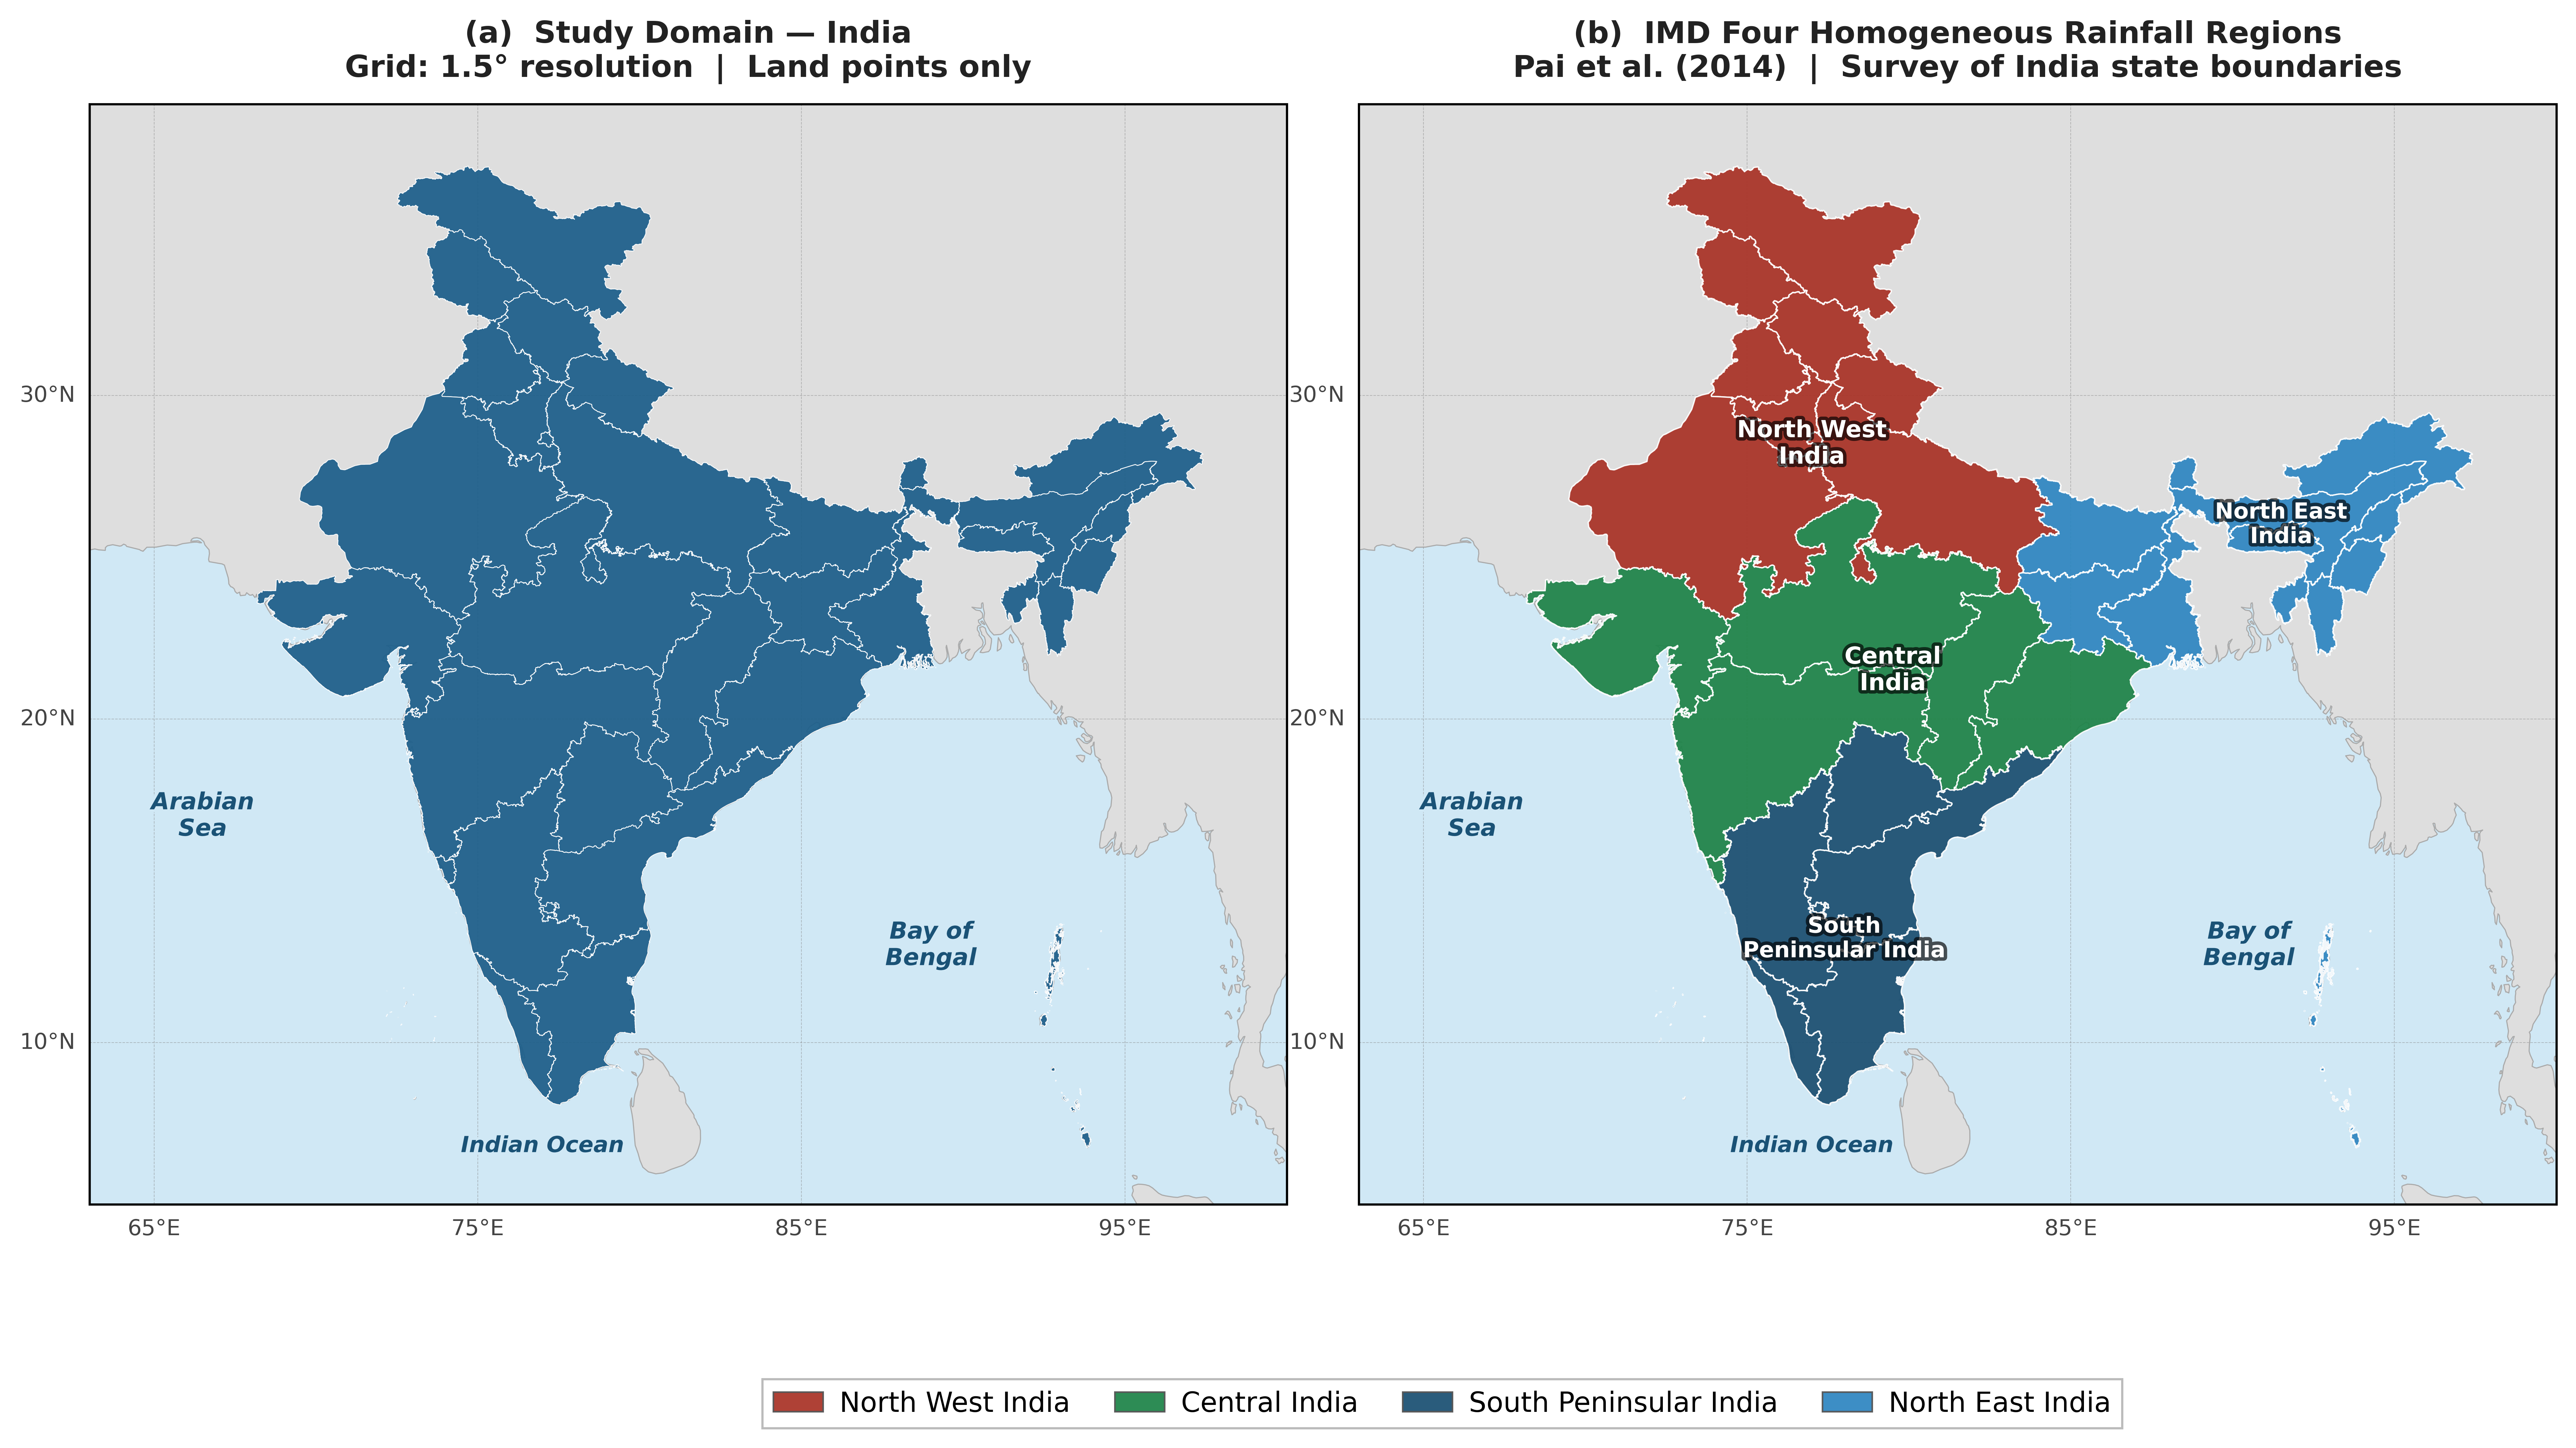
\includegraphics[width=\linewidth]{figs/fig01_domain.png}
  \caption{The India study domain and analysis regions. (a)~The
  verification domain ($5^{\circ}$--$38^{\circ}$N,
  $65^{\circ}$--$100^{\circ}$E) on the common $1.5^{\circ}$ grid; only
  land points (India shaded blue, ocean light blue) are retained for the
  area-aggregated scores. (b)~The four IMD homogeneous rainfall regions
  used in the regional analysis---Northwest, Central, South Peninsula,
  and East/Northeast India---delineated by Survey-of-India state
  boundaries following \citet{pai2014}. All 13 weekly forecasts span
  1~January--26~March~2026.}
  \label{fig:domain}
\end{figure}

\subsection{Forecast data}\label{sec:fcstdata}

Weekly initialized forecasts are collected from the four systems
summarized in Table~\ref{tab:models} for the 13 initialization dates
listed in Section~\ref{sec:weeks}. ECMWF and NCEP forecasts are
obtained from the WWRP/WCRP S2S database \citep{vitart2017}, using the
perturbed-forecast ensembles. Spire AI-S2S forecasts are provided by
Spire Global under a research arrangement. FuXi-S2S forecasts are
generated from the publicly released model, initialized from ERA5
analyses at 00~UTC on each start date \citep{chen2024}.

\begin{table}[t]
  \caption{Verification dataset and protocol summary.}
  \label{tab:verif}
  \centering
  \small
  \begin{tabular}{ll}
    \toprule
    Property & Specification \\
    \midrule
    Reference dataset        & ERA5 \citep{hersbach2020} \\
    Variables                & Precipitation, Z500 \\
    Native resolution        & ERA5 hourly/daily (ARCO for tp, t2m) \\
    Verification grid        & $1.5^{\circ}$ common grid (conservative remapping) \\
    Temporal aggregation     & Hourly/daily $\rightarrow$ daily (00--00 UTC) $\rightarrow$ weekly \\
    Verification period      & 1 January -- 6 May 2026 \\
    Observed climatology     & 30-yr ERA5 day-of-year mean, 1990--2019 (Section~\ref{sec:anom}) \\
    Spatial mask             & Indian land points, $\cos\varphi$ area weights \\
    \bottomrule
  \end{tabular}
\end{table}

\section{Methodology}\label{sec:method}

\subsection{Initialization dates and weekly lead windows}\label{sec:weeks}

Thirteen initializations at weekly intervals span the JFM 2026 season:
1, 8, 15, 22, and 29 January; 5, 12, 19, and 26 February; and 5, 12,
19, and 26 March 2026. All forecasts are taken from the 00~UTC cycle:
the AI systems (SPIRE and FuXi-S2S) are initialized from the 00~UTC ERA5
analysis, and the ECMWF and NCEP forecasts are the 00~UTC runs archived
on the S2S database. Each forecast is partitioned into six nonoverlapping
weekly lead windows---week~1 to forecast days 1--7, week~2 to days 8--14,
and so on through week~6 (days 36--42), where day~1 denotes the first
24~h after initialization. Skill is evaluated for weeks 1--6 where the
forecast horizon permits (Table~\ref{tab:models}); the deterministic
score tables (Tables~\ref{tab:acc}--\ref{tab:rmse}) summarize weeks 1--4,
and the figures extend to week~6.

Because the systems deliver the two variables in different native forms,
each is reconciled to a common weekly quantity before scoring.

\textbf{Z500.}
Every system---including the ERA5 reference---archives geopotential
($\Phi$, units J\,kg$^{-1}$) or geopotential height (m). We convert
ERA5 and FuXi-S2S geopotential to geopotential height by dividing by
the standard gravity $g = 9.80665$\,m\,s$^{-2}$; ECMWF, NCEP, and
Spire already deliver geopotential height directly. For each lead window,
the daily height values are averaged to a weekly-mean field (m).

\textbf{Precipitation.}
All systems are reduced to a weekly-mean daily rate (mm\,day$^{-1}$)
before scoring. The four systems handle precipitation differently:
\begin{itemize}
  \item \textit{Spire AI-S2S} delivers daily precipitation totals
    (mm\,day$^{-1}$); these are averaged over the seven days of the
    lead window.
  \item \textit{FuXi-S2S} provides precipitation as a mean rate in
    mm\,h$^{-1}$, roughly 24 times smaller than a daily total.
    Each daily value is multiplied by 24 to convert to
    mm\,day$^{-1}$, then the seven days are averaged
    (Section~\ref{sec:metrics}).
  \item \textit{ECMWF and NCEP} archive precipitation as a running
    cumulative accumulation from initialization (mm), i.e.\ the total
    accumulated from day~0. The weekly-mean rate is recovered by
    differencing the cumulative totals at the last day ($d_e$) and the
    day before the window opens ($d_s - 1$), then dividing by the
    number of days $N$:
    \begin{equation}
      \overline{P}_{w} = \frac{\mathrm{TP}(d_e) - \mathrm{TP}(d_s-1)}{N},
      \label{eq:deaccum}
    \end{equation}
    where $d_s$ and $d_e$ are the start and end forecast-day indices
    of the week (e.g.\ $d_s=8$, $d_e=14$ for week~2), and
    $\mathrm{TP}(d_s-1)=0$ for week~1.
  \item \textit{ERA5 reference:} the precipitation truth is constructed
    from hourly ARCO-ERA5 fields summed to true 24-h daily totals
    (00--00~UTC), then averaged over the lead window. The construction
    of this reference and its importance for avoiding a known
    under-counting artifact are detailed in Section~\ref{sec:metrics}.
\end{itemize}
All weekly fields are then remapped to the common $1.5^{\circ}$ grid
(Section~\ref{sec:grid}) and converted to anomalies
(Section~\ref{sec:anom}).

\subsection{Common grid}\label{sec:grid}

All forecasts and the ERA5 reference are remapped to a common
$1.5^{\circ}$ latitude--longitude grid (matching the coarsest delivered
system, the S2S archive grid) prior to verification, so that no
high-resolution system is penalized for representing fine scales the
others cannot. Bilinear interpolation is used for the continuous fields;
precipitation is remapped so as to preserve area-integrated totals.

\subsection{Climatologies and anomaly definition}\label{sec:anom}

Both forecast and observed anomalies are defined by removing a single
common climatology: a 30-year (1990--2019) ERA5 day-of-year climatology,
evaluated for the calendar days of each verifying week and applied
identically to every system and to the ERA5 reference. Because this
observed baseline is computed over three decades \emph{independent} of
the 2026 verification season, it avoids the amplitude inflation that an
in-sample seasonal mean would introduce, in keeping with standard WMO
practice for anomaly verification. System-specific reforecast (hindcast)
climatologies were not available for the real-time configurations
evaluated here, so a lead-dependent model-drift correction could not be
applied. The identical observed baseline is nonetheless subtracted from
all four systems and from the reference, so no system is advantaged
relative to another, and our headline metric---the spatially
\emph{centered} pattern correlation (Eq.~\ref{eq:acc})---measures
agreement in the \emph{shape} of the anomaly field and is insensitive to
any residual uniform mean offset.

\subsection{Ensemble treatment}\label{sec:ens}

Verification targets the ensemble mean of each system, computed
identically across all four: the SPIRE provider-supplied ensemble mean,
the FuXi-S2S 11-member mean, and the ECMWF and NCEP perturbed-member
(PF) means (100 and 15 members, respectively; member counts in
Table~\ref{tab:models}). Ensemble means from unequal ensemble sizes are
not strictly comparable, because larger ensembles damp unpredictable
variance more effectively; this asymmetry favours the larger ECMWF and
SPIRE ensembles at longer leads and is carried as a caveat
(Section~\ref{sec:limitations}). Beyond the ensemble mean, we
additionally place all four systems on a common probabilistic footing
and assess their calibration (Section~\ref{sec:prob_methods}).

\section{Forecast Models}\label{sec:models}

We evaluate six S2S forecast systems spanning three dynamical NWP ensembles and three
AI-based systems. Table~\ref{tab:models} summarizes their configurations; the dynamical
systems (ECMWF, UKMO, NCEP) are obtained from the WWRP/WCRP S2S database
\citep{vitart2017}, while the AI systems (Spire, FuXi-S2S, DLESyM) were received
directly from their respective providers. All six systems are evaluated over JFM~2026;
five (excluding Spire) participate in the extended JJAS~2019 case study
(Section~\ref{sec:jjas2019}).

\begin{table}[t]
  \caption{Forecast systems evaluated, as configured for JFM~2026.
  ``Native res.'' is the model's own horizontal grid; all systems are
  regridded to the common $1.5^{\circ}$ verification grid before scoring
  (Section~\ref{sec:grid}). CF\,=\,control forecast; PF\,=\,perturbed-forecast
  members. Spire AI-S2S is delivered as ensemble mean and standard deviation
  rather than individual members. ``Horizon'' is the maximum forecast lead.
  All four systems are initialized on the 13 weekly dates of
  Section~\ref{sec:weeks}; ensemble sizes, horizons, and grids were confirmed
  from the delivered files.}
  \label{tab:models}
  \centering
  \small
  \setlength{\tabcolsep}{6pt}
  \begin{tabular}{llcccl}
    \toprule
    System & Type & Native res. & Members & Horizon & Seasons \\
    \midrule
    Spire AI-S2S    & AI (data-driven)       & $0.5^{\circ}$          & mean\,$+$\,s.d.      & 46\,d & JFM\,2026 \\
    FuXi-S2S        & AI (data-driven)       & $1.5^{\circ}$          & 1\,CF\,$+$\,10\,PF   & 42\,d & JFM\,2026, JJAS\,2019 \\
    DLESyM          & AI (diffusion-based)   & $0.25^{\circ}$         & 80\,PF               & 48\,d & JFM\,2026, JJAS\,2019 \\
    ECMWF ext-range & Dynamical, coupled     & Tco319 ($\sim$36\,km)  & 100\,PF              & 46\,d & JFM\,2026, JJAS\,2019 \\
    UKMO GloSea6    & Dynamical, coupled     & N216 ($\sim$60\,km)    & 1\,CF\,$+$\,3\,PF    & 60\,d & JFM\,2026, JJAS\,2019 \\
    NCEP CFSv2      & Dynamical, coupled     & T126 ($\sim$100\,km)   & 15\,PF               & 44\,d & JFM\,2026, JJAS\,2019 \\
    \bottomrule
  \end{tabular}
\end{table}

\subsection{ECMWF extended-range ensemble}\label{sec:ecmwf}

The ECMWF Integrated Forecasting System (IFS) extended-range ensemble
\citep{vitart2014} is a fully coupled atmosphere--ocean--land--sea-ice
model run twice weekly (Mondays and Thursdays) to day~46. For the JFM~2026
period we use the 00~UTC Thursday runs archived on the S2S database
\citep{vitart2017} at $1.5^{\circ}$ (interpolated from the native Tco319,
$\approx$36~km, spectral grid). Each initialization provides 100
perturbed-forecast (PF) members generated by singular-vector and
stochastic-physics perturbations; we use the 100-member ensemble mean for
deterministic scores and the full ensemble for probabilistic verification.
The IFS extended-range configuration also provides on-the-fly reforecasts
(11 members, 20 years) used by ECMWF to generate lead-dependent model
climatologies; in this study, anomalies are instead computed against the
common 30-year ERA5 climatology (Section~\ref{sec:anom}) to ensure a fair
cross-system comparison.

\subsection{NCEP CFSv2}\label{sec:ncep}

The NCEP Climate Forecast System version~2 \citep{saha2014} is a fully
coupled atmosphere--ocean--land system operational since 2011. The
atmosphere is resolved at T126 ($\approx$100~km) with 64 hybrid sigma-pressure
levels; the ocean component is MOM4 at $0.25$--$0.5^{\circ}$ resolution.
Forecasts are archived on the S2S database \citep{vitart2017} at
$1.5^{\circ}$ to a 44-day horizon. From each 00~UTC initialization we use
the 15-member perturbed-forecast ensemble. A dedicated
1999--2010 reforecast set (four members per start date) provides the
provider-native model climatology, although---as with ECMWF---anomalies
here are computed from the common ERA5 climatology.

\subsection{Spire AI-S2S}\label{sec:spire}

Spire AI-S2S \citep{spire2026} is a commercially produced, ML-based
subseasonal forecasting system developed by Spire Global. Forecasts are
delivered on a $0.5^{\circ}$ global grid at daily temporal resolution to a
46-day horizon, initialized from 00~UTC ERA5 analyses. Rather than
distributing individual ensemble members, the system supplies ensemble
summary products: the ensemble mean and standard deviation (used here for
both deterministic and probabilistic verification), together with
exceedance-probability and percentile products that we do not use in this
study. The system produces daily total precipitation (mm\,day$^{-1}$) and
geopotential height, among other fields; no unit conversion is required for
precipitation. We received forecasts for all 13 weekly JFM~2026
initializations under a research data-use agreement.

\subsection{FuXi-S2S}\label{sec:fuxi}

FuXi-S2S \citep{chen2024} is an ML subseasonal forecasting system built on
the FuXi transformer architecture trained on ERA5 reanalysis. The published
system generates 42-day global forecasts on a $1.5^{\circ}$ grid and has been
shown to outperform the ECMWF S2S baseline for week-3--4 global precipitation
\citep{chen2024}. The forecasts available to us for JFM~2026 comprise an
11-member ensemble (1~CF\,$+$\,10~PF), initialized from 00~UTC ERA5 fields;
we use the ensemble mean for deterministic scores and the member spread for
probabilistic verification. The FuXi-S2S precipitation channel is delivered
as a mean rate (mm\,h$^{-1}$) rather than a daily total and is multiplied by
24 before scoring to convert to mm\,day$^{-1}$ (Section~\ref{sec:metrics}).
Because both AI systems (Spire and FuXi-S2S) are initialized directly from
ERA5, they share the verifying reanalysis's initial state, an advantage not
available to the dynamical systems which use their own model analyses; the
implications of this initialization asymmetry are discussed in
Section~\ref{sec:limitations}.

\subsection{UKMO GloSea6}\label{sec:ukmo}

The UK Met Office Global Seasonal Forecasting System version~6
\citep[GloSea6;][]{maclauchlan2014} is a fully coupled atmosphere--ocean--land
system run twice weekly (Mondays and Thursdays) to a 60-day horizon. The
atmospheric component is the Met Office Unified Model (MetUM) at $\sim$60~km
(N216) resolution; the ocean component is the NEMO model at $0.25^\circ$.
For this study we use the 00~UTC Thursday runs archived on the S2S database at
$1.5^\circ$, comprising one control forecast (CF) plus three perturbed members (PF),
giving a four-member ensemble per initialization. The small ensemble size limits
probabilistic skill (CRPS, Brier score) but provides full deterministic
verification (ACC, RMSE). UKMO delivers total precipitation as a running cumulative
accumulation from initialization (kg\,m$^{-2}$, equivalent to mm), processed
identically to ECMWF using the de-accumulation formula (Eq.~\ref{eq:deaccum}).
Geopotential height is delivered directly in gpm and requires no unit conversion.
2-m temperature data are available in the archive but contain only a single forecast
step due to the data retrieval configuration; UKMO T2M is therefore excluded from
the verification and all rankings.

\subsection{DLESyM}\label{sec:delysm}

DLESyM (Deep Learning Earth System Model; \citealt{cresswellclay2024}) is a
diffusion-based coupled atmosphere--land--ocean ML system trained on ERA5 and
CMIP6 simulations. Forecasts are run on a $0.25^\circ$ global grid to a 48-day
horizon and delivered as a large 80-member ensemble, making DLESyM the
highest-resolution and highest-member-count system in our comparison. The 80-member
ensemble is particularly advantageous for probabilistic verification.

DLESyM delivers 6-hourly output; for verification we compute daily means (averaging
over four 6-hourly steps) before aggregating to weekly-mean fields. The z500 variable
is stored as geopotential ($\Phi$, m$^2$\,s$^{-2}$) and is divided by
$g = 9.80665$\,m\,s$^{-2}$ to obtain geopotential height (gpm), consistent with the
treatment of ERA5. 2-m temperature is stored in Kelvin. DLESyM does not currently
provide a precipitation channel; it therefore participates in Z500 and T2M
verification only and is excluded from all precipitation rankings.

Forecasts are stored as per-initialization zarr archives indexed by initialization
date. Three stores were identified as corrupted (all-zero values for
\texttt{jjas2019/20190603}; missing zarr for \texttt{jjas2019/20190617} and
\texttt{jjas2025/20250612}) and are excluded from the comparable-init sets; an
automated guard rejects any store that reads as all-zero at the first lead, flagging
it rather than silently contributing erroneous skill scores.

\section{Verification Framework}\label{sec:verif}

Let $f'_{i,t,\ell}$ denote the ensemble-mean forecast anomaly at land
grid point $i$, initialization $t$ ($t=1,\dots,T$; $T=13$), and weekly
lead $\ell\in\{1,2,3,4\}$, and let $o'_{i,t,\ell}$ denote the
corresponding ERA5 anomaly for the same verifying week. Area weights
are $w_i=\cos\varphi_i$, with sums taken over the land mask of
Fig.~\ref{fig:domain}.

\subsection{Metrics}\label{sec:metrics}

The Anomaly Correlation Coefficient (ACC; also referred to as the
Anomaly Pattern Correlation Coefficient, APCC, in the WMO verification
guidelines) at lead $\ell$ is the cosine-latitude-weighted, spatially
\emph{centered} Pearson correlation of forecast and observed anomaly
fields, computed per initialization and averaged over the season.
Following WMO (2023), both anomalies are spatially centred before
correlating---the cosine-weighted spatial mean of the anomaly field is
removed---so that a spatially uniform offset does not inflate the score.
Formally,
\begin{equation}
  \mathrm{ACC}(\ell) \;=\; \frac{1}{T}\sum_{t=1}^{T}
  \frac{\sum_i w_i\,(f'_{i,t,\ell}-\overline{f'}_{t,\ell})\,
                     (o'_{i,t,\ell}-\overline{o'}_{t,\ell})}
       {\sqrt{\sum_i w_i\,(f'_{i,t,\ell}-\overline{f'}_{t,\ell})^{2}}\,
        \sqrt{\sum_i w_i\,(o'_{i,t,\ell}-\overline{o'}_{t,\ell})^{2}}}\,,
  \label{eq:acc}
\end{equation}
where $\overline{x}_{t,\ell}=\big(\sum_i w_i x_{i,t,\ell}\big)/\sum_i w_i$
denotes the cosine-weighted spatial mean over land points. This is the
exact estimator implemented in the verification code; the seasonal
average is taken on the raw per-initialization correlations (not on
Fisher-$z$ transforms). The root-mean-square error is
\begin{equation}
  \mathrm{RMSE}(\ell) \;=\; \frac{1}{T}\sum_{t=1}^{T}
  \sqrt{\frac{\sum_i w_i\,\bigl(f_{i,t,\ell}-o_{i,t,\ell}\bigr)^{2}}
             {\sum_i w_i}}\,,
  \label{eq:rmse}
\end{equation}
evaluated on the weekly-mean fields in their native units
(mm\,day$^{-1}$ for precipitation, m for Z500, K for temperature), and
the mean bias is
\begin{equation}
  \mathrm{Bias}(\ell) \;=\; \frac{1}{T}\sum_{t=1}^{T}
  \frac{\sum_i w_i\,\bigl(f_{i,t,\ell}-o_{i,t,\ell}\bigr)}
       {\sum_i w_i}\,,
  \label{eq:bias}
\end{equation}
in the field's native units. \textbf{Precipitation reference.} Both
variables are verified with the full metric set (ACC, RMSE, and bias).
We emphasize one methodological point that materially affects the
precipitation results: the precipitation reference must be a true
24-hour daily accumulation. An earlier version of this analysis used an
ERA5 precipitation field archived as a single 6-hour accumulation per
day, which under-represents the daily total by roughly an order of
magnitude and, because it shares the native scale and structure of the
reanalysis-trained AI output, spuriously inflated the apparent
precipitation skill of the system trained to emulate ERA5. We therefore
construct the precipitation reference from hourly ERA5 obtained from the
Analysis-Ready, Cloud-Optimized ERA5 archive
\citep[ARCO-ERA5;][]{carver2023}, summed to true 24-hour daily totals
($\approx$0.8--1.4~mm\,day$^{-1}$ domain mean over the season),
consistent in scale with the systems that report daily-total
precipitation. All precipitation scores reported below use this
corrected reference.

\textbf{Precipitation unit harmonization.} A second, independent
precipitation issue concerns the \emph{forecast} units. The FuXi-S2S
\texttt{tp} channel is archived as a mean precipitation rate
(mm\,h$^{-1}$): its values are flat across lead day (confirming a rate
rather than an accumulation) and roughly twenty times smaller than the
daily totals of the other systems, which are already in mm\,day$^{-1}$.
We therefore multiply the FuXi-S2S precipitation field by 24 to convert
it to a daily total before any scoring; SPIRE, ECMWF, and NCEP require no
such adjustment (their domain-mean week-1 precipitation, 0.82, 0.77, and
0.84~mm\,day$^{-1}$, already matches the observed 0.82). This
harmonization is not merely cosmetic for the anomaly correlation of
Eq.~(\ref{eq:acc}): because the anomaly is formed by subtracting a
climatology computed on the true daily scale, an un-converted FuXi-S2S
field yields an almost spatially uniform negative anomaly that collapses
its week-1 precipitation ACC to an artificial 0.43; after conversion the
same field scores 0.76, a physically sensible value. Pattern
correlations of the other systems and of all non-precipitation variables
are unaffected by this step.

\textbf{Point-by-point verification.} As a distribution-level complement
to the domain-aggregated scores, we also report the joint density of
forecast and observed values pooled over all 13 initializations, all six
lead weeks (forecast days 1--42), and all land grid points
(Fig.~\ref{fig:scatter}). For each variable--system pair this yields
$\approx$26{,}000 paired values, summarized by the coefficient of
determination $R^{2}$ (the squared Pearson correlation of the pooled
pairs), the mean absolute error (MAE), and the bias; precipitation and
Z500 anomaly are shown in physical units and temperature as the absolute
field. Because the leads are pooled, this diagnostic characterizes
overall agreement rather than lead-dependent skill, which is reported
separately in Fig.~\ref{fig:acc_lead}.

For the spatial skill maps, the local temporal pattern correlation at
each grid point is the correlation, across the $T=13$ initializations,
between forecast and observed weekly Z500 anomalies. With so few samples
these maps are necessarily noisy and are interpreted qualitatively.

\subsection{Reference forecasts}\label{sec:baselines}

Two reference forecasts contextualize all scores: (i)~climatology
(zero anomaly), for which the ACC of Eq.~(\ref{eq:acc}) is undefined
and the anomaly RMSE equals the observed anomaly standard deviation;
and (ii)~persistence, defined as the observed anomaly of the week
immediately preceding initialization, applied at all leads.
The persistence baseline is shown in Fig.~\ref{fig:mme} (Appendix).

\subsection{Uncertainty estimation}\label{sec:uncertainty}

Confidence intervals for all aggregate scores are estimated by
bootstrap resampling of the 13 initialization dates (1000 resamples;
2.5th--97.5th percentile, i.e.\ 95\%, intervals). Differences between
systems are assessed by a paired bootstrap: for each resample of the
initialization dates we recompute the difference in the seasonal-mean
score between the two systems on the \emph{same} resampled dates, and we
call a difference significant when the resulting 95\% interval excludes
zero (equivalently, a two-sided $p<0.05$). Pairing on initialization date
removes the large init-to-init variability common to both systems and is
the basis for significance assessments of paired differences. Given
$T=13$, only large differences are expected to be distinguishable, and
all statements of relative skill in Section~\ref{sec:results} should be
read with this caveat.

\subsection{Interpreting deterministic scores for smooth forecasts}
\label{sec:smoothing}

Ensemble means---and, by construction, many ML forecasts---are
smoother than individual realizations of the atmosphere. Deterministic
scores such as RMSE therefore structurally reward low-variance
forecasts (the ``double penalty'' effect;
\citealp{wilks2019,benbouallegue2024}). To make this effect visible we
additionally examine the ratio of forecast to observed spatial standard
deviation: all four systems markedly under-disperse precipitation
($\sigma_f/\sigma_o\approx0.5$--0.7), confirming that the modest
precipitation RMSE is partly a smoothing artifact, so we interpret RMSE
alongside ACC and bias rather than in isolation \citep{murphy1988}.

\subsection{Probabilistic verification}\label{sec:prob_methods}

Because the four systems carry very different ensemble information
(Spire delivers ensemble mean\,+\,s.d.; FuXi-S2S, ECMWF, and NCEP
provide 11, 100, and 15 members respectively), we place them on a common
footing by treating each as a Gaussian forecast with the ensemble mean
$\mu$ and the ensemble spread (standard deviation) $\sigma$ at each grid
point and lead
\emph{day}. The continuous ranked probability score then has the
closed form
\begin{equation}
  \mathrm{CRPS}(\mu,\sigma,y) = \sigma\!\left[\omega\,(2\Phi(\omega)-1)
  + 2\phi(\omega) - \tfrac{1}{\sqrt{\pi}}\right],\quad \omega=\tfrac{y-\mu}{\sigma},
  \label{eq:crps}
\end{equation}
with $y$ the observation and $\Phi,\phi$ the standard-normal CDF and PDF
\citep{gneiting2007}. Scores are computed per day, then averaged over the
land points and the days of each lead week. The skill score
$\mathrm{CRPSS}=1-\mathrm{CRPS}/\mathrm{CRPS}_{\mathrm{clim}}$ is taken
against a Gaussian climatological reference whose mean and standard
deviation are estimated from the full ERA5 daily precipitation (or Z500)
record at each grid point. Calibration is summarized by the spread-skill
ratio $\mathrm{SSR}=\overline{\sigma}/\mathrm{RMSE}(\mu)$, which equals
one for a perfectly reliable ensemble and is below one when the ensemble
is overconfident. Reliability is assessed for the heavy-rain event
(precipitation $>1$~mm\,day$^{-1}$) using the Gaussian exceedance
probability $P(y>1)=1-\Phi\!\left(\tfrac{1-\mu}{\sigma}\right)$.
Computing all scores at the daily level makes the SPIRE spread (a daily
ensemble standard deviation) directly comparable to the member spreads of
the other systems.

% ===================================================================
% RESULTS
% ===================================================================
\section{Results}\label{sec:results}

\subsection{Large-scale circulation (Z500) skill}\label{sec:lead_skill}

SPIRE and ECMWF demonstrate the strongest large-scale circulation skill
over India (Fig.~\ref{fig:acc_lead}c,d). At week~1 both attain a Z500
ACC of 0.94, with NCEP close behind (0.92) and FuXi-S2S lower (0.82).
At week~2 SPIRE leads all systems (0.87), ahead of ECMWF (0.84), NCEP
(0.63), and FuXi-S2S (0.50), and at week~3 SPIRE (0.75) again leads
ECMWF (0.77)---the two are essentially tied---while FuXi-S2S collapses
to near zero (0.04). RMSE tells a consistent story
(Fig.~\ref{fig:acc_lead}d): at week~1 ECMWF is sharpest (8.4~m),
followed by FuXi-S2S (9.0~m), SPIRE (13.8~m), and NCEP (17.6~m); but
FuXi-S2S's RMSE degrades rapidly, and by weeks~5--6 SPIRE achieves the
\emph{lowest} RMSE of all four systems (24.8--28.0~m, versus
28.8--30.0, 30.4--33.6, and 34.9--36.3~m for ECMWF, FuXi, and NCEP).
The paired SPIRE$-$FuXi comparison shows a statistically significant
week-1 advantage for SPIRE ($\Delta\mathrm{ACC}={+}0.12$, $p<0.001$).
At weeks~4--6 all systems approach low pattern skill
(ACC${\lesssim}0.6$) and differences narrow.

\begin{figure}[t]
  \centering
  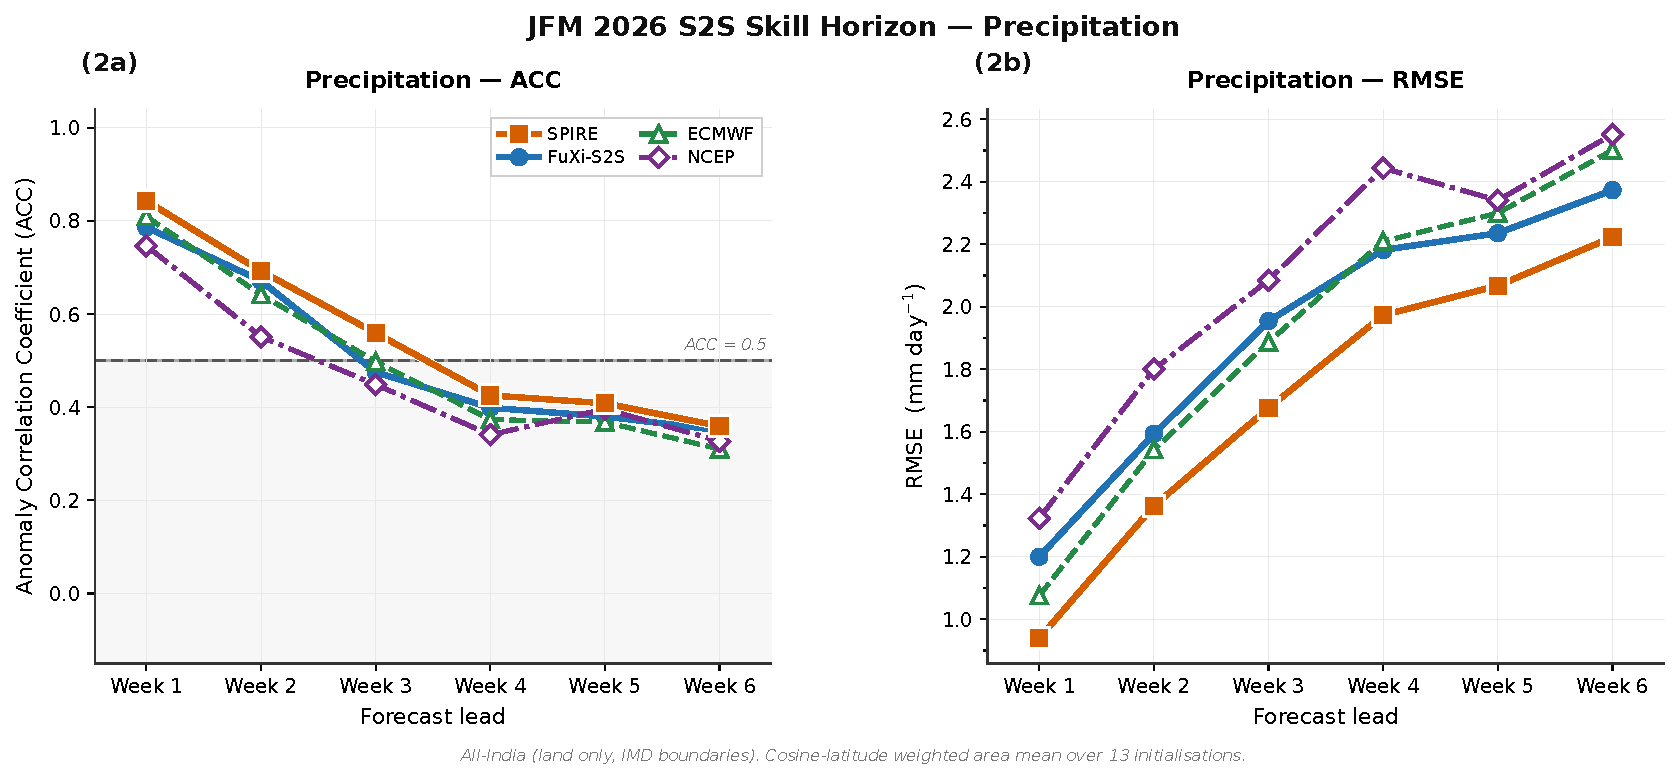
\includegraphics[width=\linewidth]{figs/fig02a_skill_tp.pdf}
  \caption{S2S skill horizon for \textbf{precipitation} over Indian land
  points, JFM 2026 (13 initializations, cosine-latitude weighted). (a)~ACC
  versus lead: SPIRE leads all systems at weeks~1--2, with all four
  crossing ACC${=}0.5$ (dashed) between weeks~2 and~3. (b)~RMSE
  (mm\,day$^{-1}$) versus lead: SPIRE has the lowest error at every week,
  growing from 0.94~mm\,day$^{-1}$ at week~1 to 2.24 at week~6.
  Precipitation is verified against true 24-hour ERA5 daily totals.
  Bootstrap 95\% CI shading over the 13 initializations.}
  \label{fig:acc_lead_tp}
  \label{fig:acc_lead}% alias for existing cross-refs
\end{figure}

\begin{figure}[t]
  \centering
  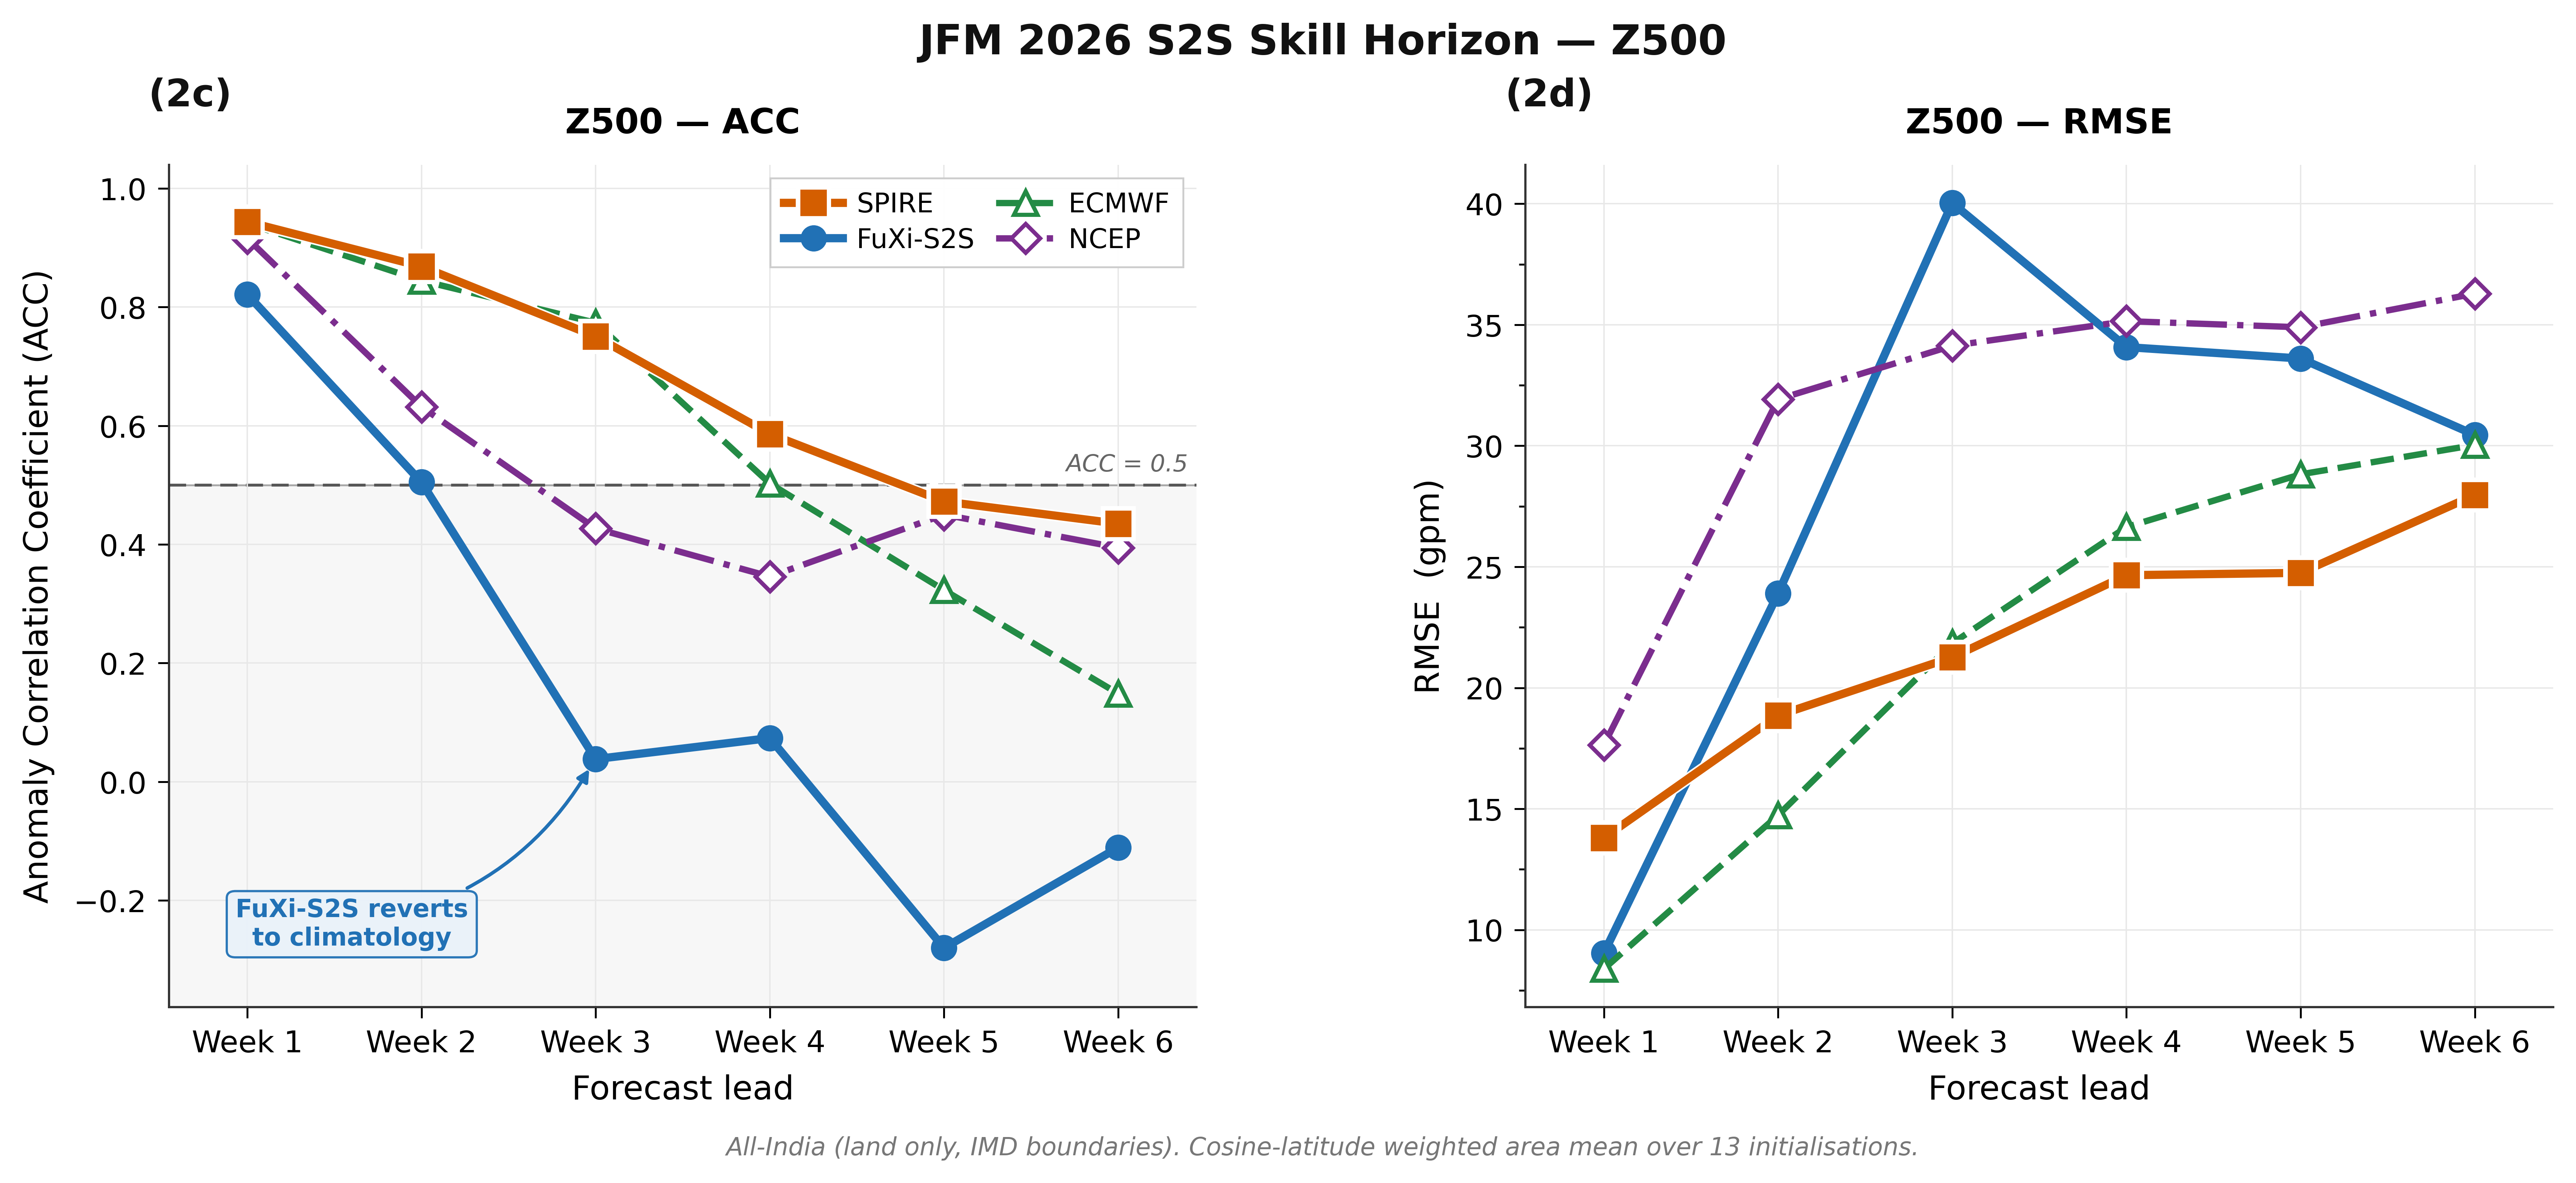
\includegraphics[width=\linewidth]{figs/fig02b_skill_z500.png}
  \caption{As Fig.~\ref{fig:acc_lead_tp} but for \textbf{Z500} (m).
  (c)~ACC: SPIRE and ECMWF are comparable at weeks~1--2 (ACC~$\approx$~0.9);
  FuXi-S2S collapses toward and below zero by week~3, consistent with
  reversion to climatology at long subseasonal leads. (d)~RMSE (m):
  SPIRE and ECMWF maintain the lowest RMSE through week~6.
  Bootstrap 95\% CI shading over the 13 initializations.}
  \label{fig:acc_lead_z500}
\end{figure}


\subsection{Precipitation skill}\label{sec:precip_skill}

Verified against the true 24-hour ERA5 daily totals
(Section~\ref{sec:metrics}), SPIRE is the most skillful precipitation
forecast of the four systems (Fig.~\ref{fig:acc_lead}a,b). Its week-1
ACC of 0.84 exceeds ECMWF (0.81), FuXi-S2S (0.79), and NCEP (0.75),
and it remains highest through week~4 (0.69, 0.56, and 0.43 at
weeks~2--4). The same ordering holds for RMSE
(Fig.~\ref{fig:acc_lead}b): SPIRE has the lowest RMSE at every lead
(0.94~mm\,day$^{-1}$ at week~1, versus 1.08 for ECMWF, 1.20 for
FuXi-S2S, and 1.32 for NCEP), and its domain-mean precipitation is
essentially unbiased against the ERA5 reference
($+0.01$~mm\,day$^{-1}$ at week~1). The paired SPIRE$-$FuXi difference is significantly positive for
precipitation through week~3 (paired bootstrap, $p<0.05$).

ECMWF and FuXi-S2S are close competitors for second place, with
week-1 correlations of 0.81 and 0.79 that are statistically
indistinguishable. NCEP CFSv2 is the weakest system at short lead (0.75
at week~1), though the four systems converge by weeks~5--6 (ACC
0.31--0.41). FuXi-S2S carries a modest dry bias
($-0.11$~mm\,day$^{-1}$ at week~1, growing to $-0.35$~mm\,day$^{-1}$
at week~4), consistent with the smoothing of extreme rainfall expected of
an MSE-trained AI model, while ECMWF and NCEP are also slightly dry
($-0.07$ and $-0.15$~mm\,day$^{-1}$ at week~1). We emphasize that the
competitive FuXi-S2S ranking emerges only after the precipitation
reference and units are reconciled (Section~\ref{sec:metrics}): the
FuXi-S2S \texttt{tp} channel is archived as a mean precipitation rate
(mm\,h$^{-1}$), not a daily total, and multiplying by 24 restores it to
a physically sensible, competitive value; without this step the anomaly
correlation collapses artificially to 0.43 at week~1.

Although SPIRE leads, absolute precipitation skill decays rapidly: by
week~3 every system is below ACC~0.56, and by week~5 all are
below 0.41. The faster decay of precipitation skill relative to Z500
skill directly addresses our third question: useful predictability of the
large-scale circulation extends well beyond the horizon of useful
precipitation predictability. Tables~\ref{tab:acc} and \ref{tab:rmse}
summarize the scores.

\begin{table*}[t]
  \centering
  \small
  \caption{Land-mean, cosine-weighted ACC over India, averaged over the
  13 JFM 2026 initializations, for precipitation (top) and Z500 (bottom).
  Best system per lead in bold. Precipitation verified against true
  24-hour ERA5 daily totals.}
  \label{tab:acc}
  \setlength{\tabcolsep}{5pt}
  \begin{tabular}{lcccccc}
    \toprule
    System & Week 1 & Week 2 & Week 3 & Week 4 & Week 5 & Week 6 \\
    \midrule
    \multicolumn{7}{l}{\emph{Total precipitation}}\\
    SPIRE        & \textbf{0.84} & \textbf{0.69} & \textbf{0.56} & \textbf{0.43} & \textbf{0.41} & \textbf{0.36} \\
    FuXi-S2S     & 0.79 & 0.67 & 0.48 & 0.40 & 0.38 & 0.35 \\
    ECMWF        & 0.81 & 0.64 & 0.50 & 0.37 & 0.37 & 0.31 \\
    NCEP CFSv2   & 0.75 & 0.55 & 0.45 & 0.34 & 0.40 & 0.33 \\
    MME          & 0.82 & 0.67 & 0.51 & 0.40 & 0.40 & 0.35 \\
    \midrule
    \multicolumn{7}{l}{\emph{Z500}}\\
    SPIRE        & \textbf{0.94} & \textbf{0.87} & 0.75          & \textbf{0.59} & \textbf{0.47} & \textbf{0.44} \\
    FuXi-S2S     & 0.82 & 0.50 & 0.04          & 0.07          & $-$0.28       & $-$0.11 \\
    ECMWF        & \textbf{0.94} & 0.84 & \textbf{0.77} & 0.50 & 0.32          & 0.15 \\
    NCEP CFSv2   & 0.92 & 0.63 & 0.43          & 0.35          & 0.45          & 0.39 \\
    MME          & \textbf{0.94} & 0.84 & 0.68 & 0.53 & \textbf{0.49} & 0.39 \\
    \bottomrule
  \end{tabular}
\end{table*}

\begin{table*}[t]
  \centering
  \small
  \caption{Land-mean, cosine-weighted RMSE over India, averaged over the
  13 JFM 2026 initializations, for precipitation (mm\,day$^{-1}$; top)
  and Z500 (m; bottom). Best system per lead in bold.}
  \label{tab:rmse}
  \setlength{\tabcolsep}{5pt}
  \begin{tabular}{lcccccc}
    \toprule
    System & Week 1 & Week 2 & Week 3 & Week 4 & Week 5 & Week 6 \\
    \midrule
    \multicolumn{7}{l}{\emph{Precipitation (mm\,day$^{-1}$)}}\\
    SPIRE        & \textbf{0.94} & \textbf{1.36} & \textbf{1.68} & \textbf{1.97} & \textbf{2.07} & \textbf{2.22} \\
    FuXi-S2S     & 1.20 & 1.59 & 1.95 & 2.18 & 2.24 & 2.37 \\
    ECMWF        & 1.08 & 1.54 & 1.89 & 2.21 & 2.30 & 2.50 \\
    NCEP CFSv2   & 1.32 & 1.80 & 2.09 & 2.44 & 2.34 & 2.55 \\
    MME          & 1.03 & 1.45 & 1.79 & 2.08 & 2.14 & 2.31 \\
    \midrule
    \multicolumn{7}{l}{\emph{Z500 (m)}}\\
    SPIRE        & 13.8 & 18.9 & 21.3 & \textbf{24.7} & \textbf{24.8} & \textbf{28.0} \\
    FuXi-S2S     &  9.0 & 23.9 & 40.0 & 34.1          & 33.6          & 30.4 \\
    ECMWF        & \textbf{8.4} & \textbf{14.7} & \textbf{21.8} & 26.6 & 28.8 & 30.0 \\
    NCEP CFSv2   & 17.6 & 31.9 & 34.1 & 35.2          & 34.9          & 36.3 \\
    MME          & \textbf{6.9} & 16.8 & 24.3 & 26.1 & 27.0 & 27.8 \\
    \bottomrule
  \end{tabular}
\end{table*}

\subsection{Reference forecasts and the multi-model ensemble}
\label{sec:mme}

Two reference forecasts are included alongside the four systems
(Fig.~\ref{fig:mme}, Appendix): a persistence forecast (the observed
weekly anomaly immediately preceding initialization, applied at all
leads) and an equal-weight multi-model ensemble (MME; the mean of the
four systems). For Z500, every system beats persistence by a wide
margin---persistence ACC is only 0.48 at week~1 and 0.38 at week~3,
versus 0.94 and 0.75--0.77 for SPIRE/ECMWF---confirming that the
circulation skill is genuine and not a restatement of low-frequency
persistence. The MME is the strongest
Z500 product: its week-1 ACC (0.94) matches the best individual systems
while achieving the lowest RMSE of any forecast (6.9~m at week~1, below
ECMWF's 8.4~m). The ACC gain of the MME over the best single system
is nonetheless small ($|\Delta\mathrm{ACC}|\leq0.03$ at weeks 1--4), so
we frame the MME advantage as an error-reduction and robustness benefit
rather than a large skill gain.

For precipitation, every system beats persistence (ACC 0.49 at week~1,
0.36 at week~3): SPIRE leads at 0.84, well above the baseline at all
leads. Here, however, the MME does \emph{not} improve on the best single
system: its week-1 precipitation ACC (0.82) sits below SPIRE's 0.84,
and its RMSE (1.03~mm\,day$^{-1}$) likewise exceeds SPIRE's 0.94.
Because SPIRE is already the strongest member, equal-weight averaging
with three lower-skill systems regresses skill toward the ensemble mean.
Multi-model averaging therefore helps for Z500, where the systems are of
comparable quality, but not for precipitation; a skill-weighted
combination would be required, which $T=13$ does not support.

A complementary diagnostic is the ratio of forecast to observed
anomaly spatial standard deviation (Section~\ref{sec:smoothing}). For
Z500 this ratio falls for SPIRE from near unity at week~1 to about 0.5
by week~4, indicating that its ensemble mean is progressively smoother
than the observed field, which partly accounts for its low RMSE; FuXi-S2S
shows the opposite, with a ratio rising above 1.4, consistent with its
larger RMSE growth, while ECMWF and NCEP remain near 0.8--1.1. RMSE
differences between systems should be read in this light.

\subsection{Spatial distribution of skill}\label{sec:spatial_skill}

The local temporal Z500 anomaly correlation at each grid point (computed
across the 13 initializations, week~2) shows a consistent north--south
gradient: correlation exceeds 0.8 across the Indo-Gangetic Plain and
western-disturbance corridor in the northwest, and decays toward the
South Peninsula where week-2 Z500 skill is lower ($\sim$0.5--0.6).
SPIRE and ECMWF are nearly indistinguishable in spatial pattern, with
high and spatially uniform skill over the northern two-thirds of India.
FuXi-S2S is already weaker across the north by week~2, and NCEP shows
the broadest low-skill region extending from Central India southward.
This north--south gradient is consistent with the domain-mean ACC in
Table~\ref{tab:acc}.

\subsection{Regional skill}\label{sec:regional_skill}

Tables~\ref{tab:reg_pcc}--\ref{tab:reg_bias} give pattern skill broken
down by IMD homogeneous region (Northwest, Central, South Peninsula,
East/Northeast India), averaged over weeks~1--6.
The regional tables provide the full lead dependence by region.

For Z500 (weeks~1--6 mean, Table~\ref{tab:reg_pcc}), ECMWF and SPIRE
are near-tied over most subregions. ECMWF leads over East/Northeast
India (0.67 versus SPIRE 0.63) while SPIRE leads over Central India
(0.62 versus ECMWF 0.56). The MME is competitive everywhere
(0.55--0.67). FuXi-S2S has the lowest ACC in all four regions
(0.14--0.49), driven by its collapse at weeks~3--6. NCEP is
consistently second-weakest (0.23--0.48).

For precipitation (Table~\ref{tab:reg_pcc}), SPIRE leads in three of
four subregions (Northwest 0.47, South Peninsula 0.38, East/Northeast
0.60) and is essentially tied with ECMWF and NCEP over Central India
(0.55 vs.\ 0.56 and 0.60). Precipitation skill is highest over
East/Northeast India and lowest over the South Peninsula, reflecting the
difficulty of capturing orographic and convective rainfall at
$\sim1^\circ$ resolution. The MME adds only marginal value for
precipitation (All-India 0.53 versus SPIRE 0.55), consistent with the
domain-mean result. With four regions and 13 initializations these
regional estimates are indicative rather than definitive.
Tables~\ref{tab:reg_pcc}--\ref{tab:reg_bias} give the full week-1--6
regional scorecard for ACC, RMSE, and bias.

\begin{table*}[t]\centering
\small
\setlength{\tabcolsep}{5pt}
\caption{Region-wise ACC by IMD homogeneous region (weeks 1--6 mean,
13-init average). Best system per region in bold.}\label{tab:reg_pcc}
\begin{tabular}{lcccccc}\toprule
Region & & SPIRE & FuXi-S2S & ECMWF & NCEP & MME \\
\midrule
\multirow{5}{*}{\emph{Precipitation}} &
All India    & \textbf{0.55} & 0.51 & 0.50 & 0.47 & 0.53 \\
& Northwest    & \textbf{0.47} & 0.48 & 0.42 & 0.34 & 0.46 \\
& Central      & 0.55 & 0.45 & \textbf{0.56} & \textbf{0.60} & 0.57 \\
& S. Peninsula & \textbf{0.38} & 0.34 & 0.37 & 0.32 & 0.36 \\
& East/NE      & \textbf{0.60} & 0.56 & 0.56 & 0.55 & 0.57 \\
\midrule
\multirow{5}{*}{\emph{Z500}} &
All India    & \textbf{0.68} & 0.18 & 0.59 & 0.53 & 0.65 \\
& Northwest    & \textbf{0.57} & 0.25 & 0.52 & 0.48 & 0.55 \\
& Central      & \textbf{0.62} & 0.14 & 0.56 & 0.44 & 0.56 \\
& S. Peninsula & 0.45 & 0.41 & \textbf{0.49} & 0.23 & \textbf{0.48} \\
& East/NE      & 0.63 & 0.28 & \textbf{0.67} & 0.48 & \textbf{0.67} \\
\bottomrule
\end{tabular}\end{table*}

\begin{table*}[t]\centering
\small
\setlength{\tabcolsep}{5pt}
\caption{Region-wise RMSE by IMD homogeneous region (weeks 1--6 mean,
13-init average). Best system per region in bold. Precipitation in
mm\,day$^{-1}$; Z500 in m.}\label{tab:reg_rmse}
\begin{tabular}{lcccccc}\toprule
Region & & SPIRE & FuXi-S2S & ECMWF & NCEP & MME \\
\midrule
\multirow{5}{*}{\emph{Precipitation}} &
All India    & \textbf{1.71} & 1.92 & 1.92 & 2.09 & 1.80 \\
& Northwest    & 1.40 & 1.37 & 1.39 & 1.70 & \textbf{1.36} \\
& Central      & 0.49 & 0.50 & \textbf{0.40} & 0.41 & 0.41 \\
& S. Peninsula & \textbf{0.89} & 0.96 & 0.90 & 0.96 & 0.89 \\
& East/NE      & \textbf{3.24} & 3.89 & 3.91 & 4.03 & 3.57 \\
\midrule
\multirow{5}{*}{\emph{Z500}} &
All India    & 21.9 & 28.5 & 21.7 & 31.7 & \textbf{21.5} \\
& Northwest    & 25.6 & 39.0 & 27.9 & 35.8 & \textbf{27.6} \\
& Central      & 19.4 & 21.1 & 18.3 & 28.9 & \textbf{18.2} \\
& S. Peninsula & 13.9 & 10.9 & 9.9  & 21.5 & \textbf{9.7} \\
& East/NE      & 20.4 & 24.6 & 19.1 & 30.6 & \textbf{18.3} \\
\bottomrule
\end{tabular}\end{table*}

\begin{table*}[t]\centering
\small
\setlength{\tabcolsep}{5pt}
\caption{Region-wise mean bias (forecast minus ERA5) by IMD homogeneous
region (weeks 1--6 mean, 13-init average). Precipitation bias in
mm\,day$^{-1}$; Z500 bias in m. Value closest to zero per region in
bold.}\label{tab:reg_bias}
\begin{tabular}{lcccccc}\toprule
Region & & SPIRE & FuXi-S2S & ECMWF & NCEP & MME \\
\midrule
\multirow{5}{*}{\emph{Precipitation}} &
All India    & $\mathbf{+0.06}$ & $-0.19$ & $-0.19$ & $-0.06$ & $-0.10$ \\
& Northwest    & $+0.22$ & $+0.05$ & $\mathbf{+0.07}$ & $+0.36$ & $+0.18$ \\
& Central      & $+0.25$ & $+0.11$ & $\mathbf{-0.01}$ & $\mathbf{-0.01}$ & $+0.09$ \\
& S. Peninsula & $+0.13$ & $-0.11$ & $\mathbf{+0.04}$ & $-0.03$ & $+0.01$ \\
& East/NE      & $\mathbf{-0.81}$ & $-1.50$ & $-1.47$ & $-1.16$ & $-1.23$ \\
\midrule
\multirow{5}{*}{\emph{Z500}} &
All India    & $+8.5$  & $-16.1$ & $\mathbf{-3.6}$  & $-24.2$ & $-8.9$ \\
& Northwest    & $+6.7$  & $-31.7$ & $\mathbf{-9.0}$  & $-23.4$ & $-14.4$ \\
& Central      & $+8.1$  & $-9.4$  & $\mathbf{-2.9}$  & $-26.2$ & $-7.6$ \\
& S. Peninsula & $+10.9$ & $+1.1$ & $\mathbf{+0.8}$  & $-20.7$ & $-2.0$ \\
& East/NE      & $+10.4$ & $-18.6$ & $\mathbf{+1.2}$  & $-25.8$ & $-8.2$ \\
\bottomrule
\end{tabular}\end{table*}

\subsection{Bias analysis}\label{sec:bias}

Figure~\ref{fig:bias_lead} shows the mean bias versus lead for Z500
(panel a) and precipitation (panel b, against the true 24-hour ERA5
reference). For Z500, SPIRE carries a positive height bias
($+12.9$~m at week~1, decaying to $+6.6$~m at week~4), while FuXi-S2S
and NCEP are negatively biased (FuXi: $-1.5$ to $-28.5$~m; NCEP:
$-14.3$ to $-27.3$~m across weeks~1--4), with ECMWF closest to zero
(Table~\ref{tab:bias}). For precipitation, SPIRE is essentially unbiased
($+0.01$~mm\,day$^{-1}$ at week~1); ECMWF and NCEP carry a slight dry
bias ($-0.07$ and $-0.15$~mm\,day$^{-1}$ at week~1); FuXi-S2S has the
largest and most lead-dependent dry bias ($-0.11$~mm\,day$^{-1}$ at
week~1 growing to $-0.35$~mm\,day$^{-1}$ at week~4), consistent with
MSE-trained AI models smoothing heavy rainfall
(Section~\ref{sec:precip_skill}).

The regional bias structure (Table~\ref{tab:reg_bias}) reveals that
SPIRE's Z500 positive bias is spatially uniform across all four IMD
regions ($+7$ to $+11$~m, weeks~1--6 mean), whereas FuXi-S2S is most
strongly negative over Northwest India ($-32$~m) and near-neutral over
the South Peninsula ($+1$~m). ECMWF is the closest to zero for Z500 in
most regions. For precipitation, all systems underestimate over
East/Northeast India (a known orographic-smoothing effect at
$\sim1^\circ$ resolution), with SPIRE having the smallest deficit
($-0.81$~mm\,day$^{-1}$ versus $-1.16$ to $-1.50$~mm\,day$^{-1}$ for
the others). Over Northwest, Central, and South Peninsula India,
biases are small ($<0.25$~mm\,day$^{-1}$) for all systems.

\begin{figure}[t]
  \centering
  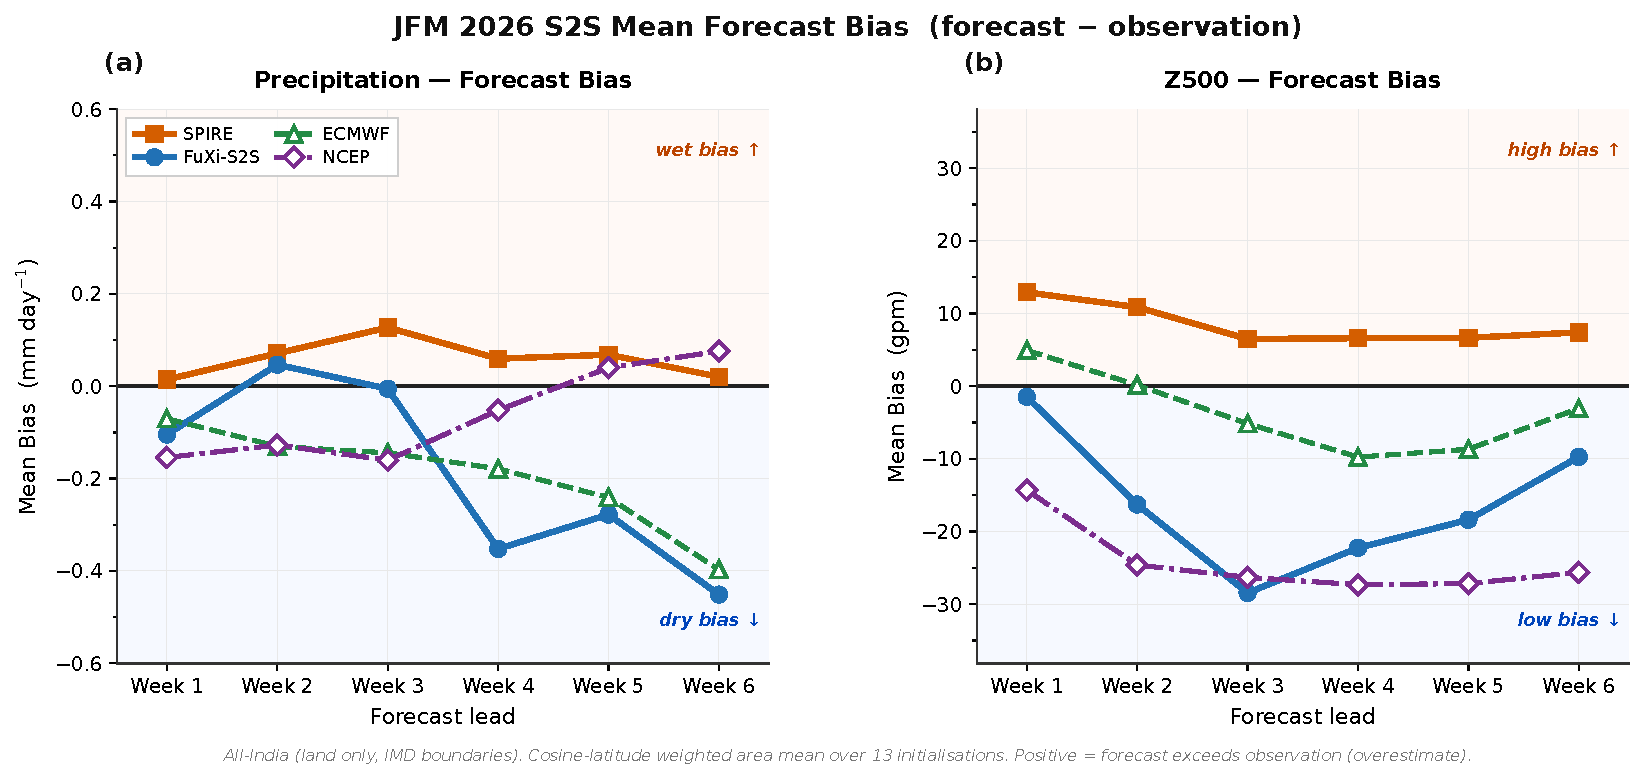
\includegraphics[width=\linewidth]{figs/fig05_bias.pdf}
  \caption{Mean bias (forecast minus ERA5) versus lead, JFM 2026, with
  bootstrap 95\% CI shading: (a)~Z500 (m) and (b)~precipitation
  (mm\,day$^{-1}$), the latter against true 24-hour ERA5 daily totals.}
  \label{fig:bias_lead}
\end{figure}

\begin{table}[t]
  \centering
  \caption{Land-mean Z500 bias (m; forecast minus ERA5), averaged over
  the 13 JFM 2026 initializations. Precipitation bias versus lead is
  shown in Fig.~\ref{fig:bias_lead}(b).}
  \label{tab:bias}
  \small
  \setlength{\tabcolsep}{5pt}
  \begin{tabular}{lcccccc}
    \toprule
    System & Week 1 & Week 2 & Week 3 & Week 4 & Week 5 & Week 6 \\
    \midrule
    SPIRE        & $+12.9$ & $+10.9$ & $+6.5$  & $+6.6$  & $+6.7$  & $+7.4$ \\
    FuXi-S2S     & $-1.5$  & $-16.3$ & $-28.5$ & $-22.3$ & $-18.4$ & $-9.7$ \\
    ECMWF        & $+4.9$  & $+0.1$  & $-5.2$  & $-9.8$  & $-8.7$  & $-3.1$ \\
    NCEP CFSv2   & $-14.3$ & $-24.6$ & $-26.3$ & $-27.3$ & $-27.2$ & $-25.6$ \\
    \bottomrule
  \end{tabular}
\end{table}

\subsection{Probabilistic skill and ensemble calibration}\label{sec:prob}

The deterministic scores use only the ensemble mean; the probabilistic
verification (Section~\ref{sec:prob_methods}) asks whether each system's
\emph{uncertainty} is trustworthy.

\paragraph{CRPSS (Fig.~\ref{fig:crpss}, Appendix; Table~\ref{tab:prob}).}
For precipitation, ECMWF leads at week~1 (CRPSS~0.62), with SPIRE
close behind (0.59) and NCEP and FuXi-S2S next (0.47 and 0.45). All
four systems beat climatology through week~4, but skill is marginal
($<$0.05) by weeks~5--6; SPIRE and NCEP reach zero at week~6.
For Z500, SPIRE leads at week~1 (0.37), well ahead of ECMWF (0.22)
and FuXi-S2S (0.18); NCEP is near zero ($-0.01$) from the outset.
By week~2, FuXi-S2S ($-0.28$) and NCEP ($-0.45$) are strongly
negative, meaning their Z500 ensembles are \emph{worse} than a
Gaussian climatological forecast. ECMWF holds positive CRPSS
through week~3 (0.08) before going negative; SPIRE retains marginal
positive skill through week~3 (0.04) and stays closest to zero
at longer leads.

\begin{table*}[t]
  \centering
  \small
  \setlength{\tabcolsep}{5pt}
  \caption{Probabilistic skill summary over India, averaged over the 13
  JFM 2026 initializations: CRPSS (top; higher is better, ${>}0$ beats
  climatology) and spread--skill ratio SSR (bottom; closest to 1.0 is
  best-calibrated). Bold marks the best CRPSS per lead; for SSR, bold
  marks the value closest to 1.0.}
  \label{tab:prob}
  \begin{tabular}{lcccccc}
    \toprule
    System & Week 1 & Week 2 & Week 3 & Week 4 & Week 5 & Week 6 \\
    \midrule
    \multicolumn{7}{l}{\emph{CRPSS --- Precipitation}}\\
    SPIRE      & 0.59          & 0.31 & 0.13          & 0.03          & 0.02          & $-$0.01 \\
    FuXi-S2S   & 0.45          & 0.20 & 0.14          & \textbf{0.17} & \textbf{0.14} & \textbf{0.14} \\
    ECMWF      & \textbf{0.62} & \textbf{0.37} & 0.15     & 0.03          & 0.03          & 0.03 \\
    NCEP CFSv2 & 0.47          & 0.27 & \textbf{0.22} & 0.05          & 0.07          & $-$0.01 \\
    \midrule
    \multicolumn{7}{l}{\emph{CRPSS --- Z500}}\\
    SPIRE      & \textbf{0.37} & 0.10    & 0.04          & \textbf{$-$0.04} & \textbf{$-$0.03} & \textbf{$-$0.11} \\
    FuXi-S2S   & 0.18          & $-$0.28 & $-$0.55       & $-$0.41          & $-$0.26          & $-$0.16 \\
    ECMWF      & 0.22          & \textbf{0.22} & \textbf{0.08} & $-$0.05       & $-$0.11          & $-$0.16 \\
    NCEP CFSv2 & $-$0.01       & $-$0.45 & $-$0.41       & $-$0.36          & $-$0.36          & $-$0.34 \\
    \midrule
    \multicolumn{7}{l}{\emph{SSR --- Precipitation (perfect = 1.00)}}\\
    SPIRE      & \textbf{0.38} & \textbf{0.68} & \textbf{0.92} & \textbf{0.90} & \textbf{0.91} & \textbf{0.84} \\
    FuXi-S2S   & 0.09          & 0.23          & 0.44          & 0.45          & 0.55          & 0.44 \\
    ECMWF      & 0.30          & 0.61          & 0.89          & 0.88          & 0.85          & 0.73 \\
    NCEP CFSv2 & 0.15          & 0.42          & 0.47          & 0.51          & 0.56          & 0.57 \\
    \midrule
    \multicolumn{7}{l}{\emph{SSR --- Z500 (perfect = 1.00)}}\\
    SPIRE      & \textbf{0.66} & 0.84          & \textbf{1.05} & 1.07          & 1.09          & \textbf{0.96} \\
    FuXi-S2S   & 0.14          & 0.36          & 0.54          & 0.77          & 0.88          & 0.87 \\
    ECMWF      & 0.31          & \textbf{0.96} & 1.15          & \textbf{1.03} & \textbf{0.97} & 0.91 \\
    NCEP CFSv2 & 0.24          & 0.48          & 0.65          & 0.69          & 0.69          & 0.67 \\
    \bottomrule
  \end{tabular}
\end{table*}

\paragraph{Spread--skill ratio (Fig.~\ref{fig:ssr}).}
The low Z500 CRPSS of FuXi-S2S and NCEP is a calibration failure.
At week~1 every system is under-dispersed (SSR~$<$~1): SPIRE is
the best calibrated for Z500 (SSR~0.66) and precipitation (0.38),
while FuXi-S2S is severely overconfident with SSR of only 0.14
and 0.09 respectively---ensemble spread roughly an order of
magnitude too small. ECMWF (SSR 0.31/0.30) and NCEP (0.24/0.15)
are intermediate. Calibration improves with lead for all systems as
ensemble spread grows: SPIRE's precipitation SSR reaches near-unity
by week~3 (0.92) and stays there through week~6 (0.84); ECMWF
reaches SSR~1 by week~3 for precipitation and week~2 for Z500, and
slightly over-disperses at weeks~3--4 (SSR~$\sim$1.15). FuXi-S2S
never achieves SSR~$>$~0.55 for precipitation across weeks~1--6,
confirming that its ensemble is structurally underconfident
regardless of lead. Figure~\ref{fig:event_spread} makes this visible
for the most anomalous event of the season: the FuXi-S2S $\pm1\sigma$
band is far narrower than SPIRE's or ECMWF's and routinely fails to
bracket the ERA5 observation for both Z500 and precipitation.

\begin{figure*}[t]
  \centering
  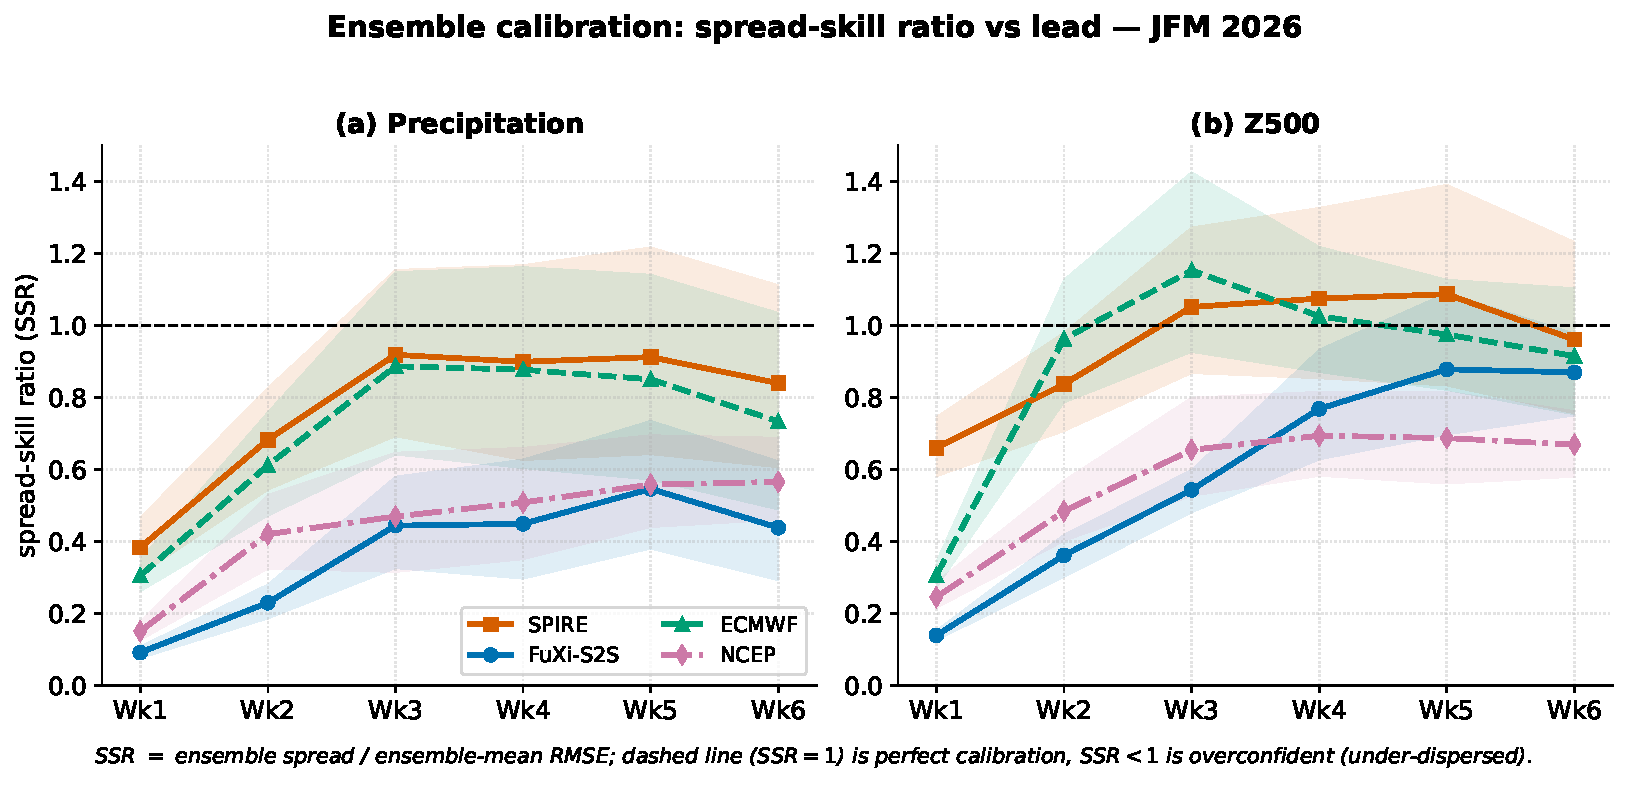
\includegraphics[width=\linewidth]{figs/fig16_spread_skill.pdf}
  \caption{Ensemble calibration: spread-skill ratio (ensemble spread
  divided by ensemble-mean RMSE) versus lead, for precipitation (a) and
  Z500 (b). The dashed line (ratio${=}1$) is perfect calibration; values
  below one indicate an overconfident (under-dispersed) ensemble. SPIRE
  is consistently closest to one; FuXi-S2S is strongly overconfident.}
  \label{fig:ssr}
\end{figure*}

\paragraph{Reliability.}
The reliability diagram for the heavy-rain threshold
($>$1~mm\,day$^{-1}$), pooling all leads and initializations,
confirms the SSR picture. SPIRE and ECMWF track closest to the
diagonal (perfect reliability), with SPIRE slightly over-forecasting
at high probabilities and ECMWF slightly under-forecasting.
FuXi-S2S lies well below the diagonal throughout, consistent with
its over-confident (too-narrow) ensemble issuing high probabilities
that verify less often than stated. NCEP is intermediate but
below-diagonal at high forecast probabilities.

\begin{figure*}[t]
  \centering
  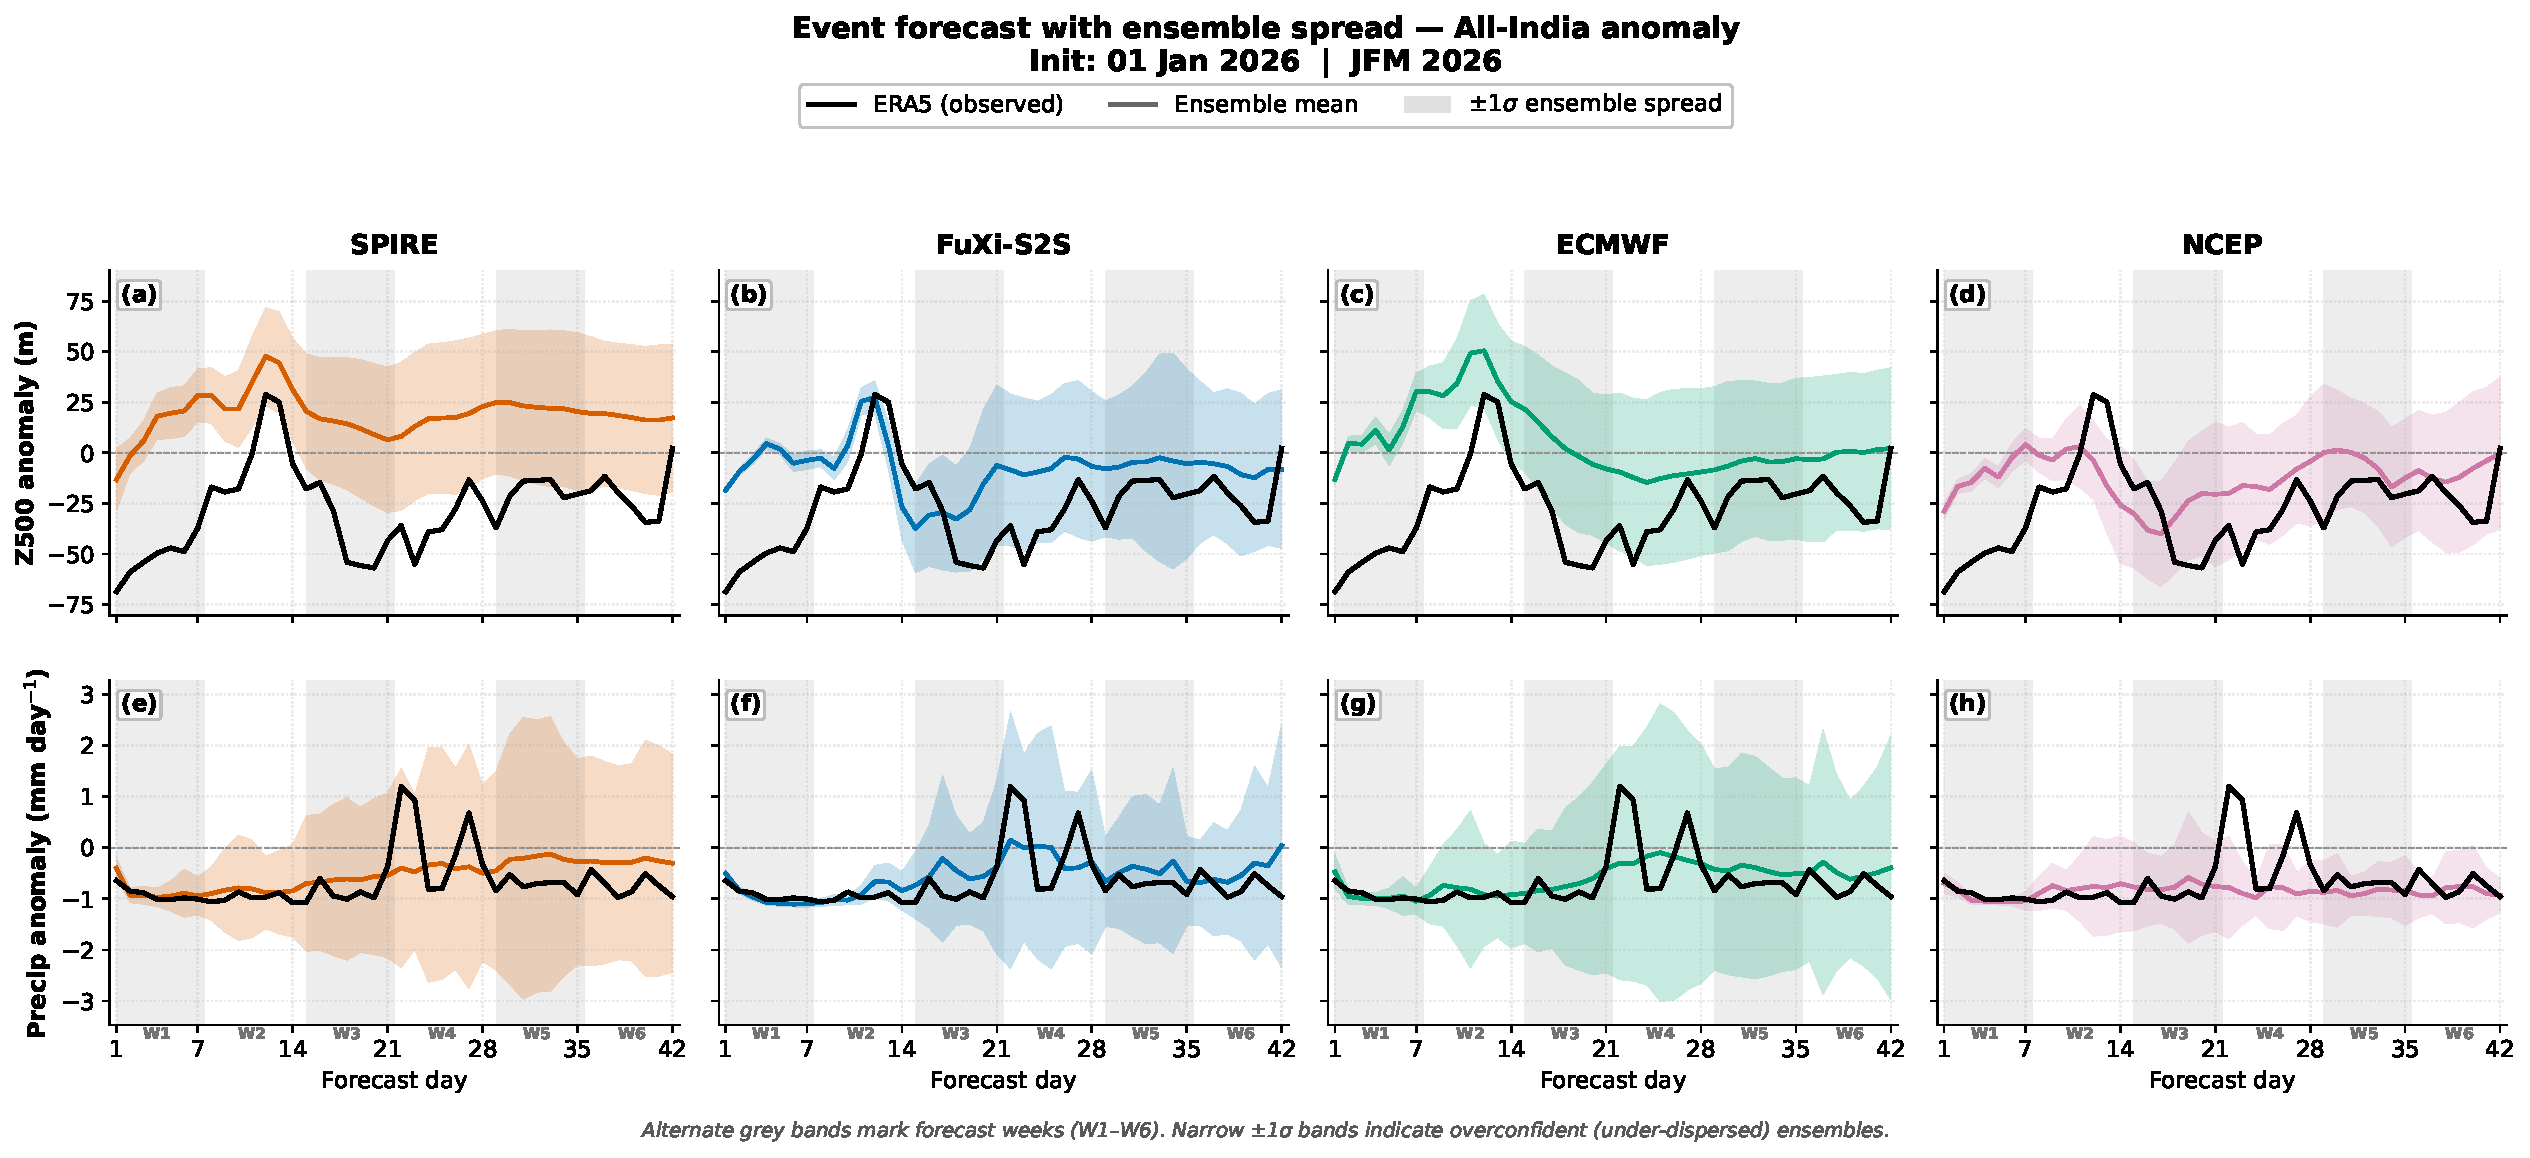
\includegraphics[width=\linewidth]{figs/fig18_event_spread.pdf}
  \caption{Ensemble spread for the most anomalous circulation event of
  JFM~2026 (initialization 1~January~2026): All-India area-averaged
  Z500 anomaly (top row, panels a--d) and precipitation anomaly (bottom
  row, panels e--h) versus forecast day, for each system. Black line is
  ERA5; coloured line is the ensemble mean; shading is $\pm1\sigma$
  ensemble spread. Grey bands mark the weekly windows (W1--W6);
  narrow shading indicates an overconfident (under-dispersed) ensemble.
  SPIRE and ECMWF maintain spread bands that broadly bracket the ERA5
  observations; FuXi-S2S is severely under-dispersed throughout.}
  \label{fig:event_spread}
\end{figure*}

\subsection{Week-6 case studies}\label{sec:case_wk6}

To show how the systems perform at the far end of the subseasonal range,
Figs.~\ref{fig:case_precip} and \ref{fig:case_z500} (Appendix) present
two independent week-6 case studies---one for precipitation and one for
Z500---each on a different initialization chosen as the one whose week-6
verifying anomaly was strongest for that field. The top row maps the
\emph{week-6 mean} anomaly (forecast days 36--42) and the bottom row
shows the All-India area-averaged anomaly through the full 42-day
forecast---ensemble mean and $\pm1\sigma$ spread---with the week-6
window shaded.

For precipitation (Fig.~\ref{fig:case_precip}), every system retains
only a weak large-scale pattern at week~6, consistent with the near-zero
precipitation ACC at that lead (Table~\ref{tab:acc}). The observed
anomaly is moderate but spatially coherent; all four ensemble means
underestimate it and their uncertainty bands are wide (SPIRE, ECMWF,
NCEP) or implausibly narrow (FuXi-S2S), consistent with the week-6 SSR
values in Table~\ref{tab:prob}.

For Z500 (Fig.~\ref{fig:case_z500}), all four systems miss the observed
positive height anomaly at week~6, illustrating that even the most
predictable field has reached the boundary of useful deterministic
skill. SPIRE and ECMWF produce the closest ensemble-mean anomaly while
FuXi-S2S's spread band frequently excludes the verifying observation,
again consistent with its underconfident calibration (SSR~$<$~0.9
throughout weeks~1--6). The full SPIRE percentile forecast for
precipitation is shown in Fig.~\ref{fig:gallery_precip} (Appendix).


\begin{figure*}[t]
  \centering
  \vspace{-0.5em}
  \includegraphics[width=\linewidth,trim=0 0 0 30,clip]{figs/fig12_scatter_weekwise_TP.png}
  \caption{Forecast--ERA5 density scatter for \textbf{precipitation anomaly}
  (mm\,day$^{-1}$) by lead week (rows: weeks~1--6) and system (columns:
  SPIRE, FuXi-S2S, ECMWF, NCEP), pooling all land grid points and 13
  initializations within each week. Colour encodes point density on a
  logarithmic scale; the blue diagonal is the 1:1 reference. Each panel
  reports $R^2$, MAE, and mean bias. SPIRE maintains the tightest
  clustering around the 1:1 line and the lowest bias at all leads.
  FuXi-S2S values are unit-harmonized ($\times24$,
  mm\,h$^{-1}\!\to$mm\,day$^{-1}$) as in Section~\ref{sec:metrics}.}
  \label{fig:scatter_tp}
  \label{fig:scatter}% alias for existing cross-refs
\end{figure*}

\begin{figure*}[t]
  \centering
  \includegraphics[width=\linewidth]{figs/fig12_scatter_weekwise_Z500.png}
  \caption{As Fig.~\ref{fig:scatter_tp} but for \textbf{Z500 anomaly} (m).
  SPIRE and ECMWF maintain a compact, near-diagonal scatter through
  week~4; FuXi-S2S shows increasing scatter and systematic spread
  compression from week~3 onward, consistent with its declining ACC and
  overconfident SSR.}
  \label{fig:scatter_z500}
\end{figure*}

\subsection{Synthesis}\label{sec:synthesis}

Taken together, the verification produces a consistent ranking across
every metric and region.

\textbf{SPIRE leads for precipitation.} Its week-1 ACC (0.84) and RMSE
(0.94~mm\,day$^{-1}$) are the best of the four systems, and this
advantage holds at every lead through week~6. It is also essentially
unbiased (All-India mean $+0.06$~mm\,day$^{-1}$, wks~1--6) and the
best-calibrated probabilistic forecast (SSR closest to 1.0 at all
leads; CRPSS 0.59 at week~1). Regionally, SPIRE tops three of four IMD
subregions for precipitation ACC (Table~\ref{tab:reg_pcc}).

\textbf{SPIRE and ECMWF are tied for Z500.} Both reach week-1 ACC 0.94.
SPIRE pulls ahead from week~3 onward in RMSE, achieving the lowest error
of any individual system at weeks~4--6 (24.7--28.0~m). ECMWF is the
best-calibrated Z500 ensemble from week~2 onward (SSR closest to 1.0).
The MME achieves the lowest Z500 RMSE overall (6.9~m at week~1) by
cancelling uncorrelated errors.

\textbf{FuXi-S2S is competitive deterministically but probabilistically
unreliable.} Once its precipitation units are harmonised ($\times24$,
Section~\ref{sec:metrics}), its week-1 ACC (0.79/0.82 for TP/Z500) is
competitive. But its ensemble spread is an order of magnitude too small
(SSR 0.09--0.14 at week~1), its Z500 CRPSS collapses to $-0.55$ by
week~3, and its bias is the largest and most lead-dependent of the four
systems for Z500 ($-28.5$~m at week~3).

\textbf{NCEP CFSv2 is the weakest system.} It has the lowest
precipitation ACC at short lead, the highest TP RMSE at all leads, and
a persistent negative Z500 bias of $-24$ to $-27$~m across weeks~2--6.
Its CRPSS for Z500 is near or below zero from the outset.

\textbf{Circulation skill outlasts precipitation skill.} Z500 ACC stays
above 0.5 through week~3--4 for SPIRE and ECMWF, while precipitation
ACC falls below 0.5 by week~3 for every system. The skill horizon for
the large-scale flow is roughly two weeks longer than for rainfall.

These rankings are consistent across metrics (ACC, RMSE, bias, CRPSS,
SSR), scales (domain-mean and four IMD subregions), and the
point-by-point scatter (Figs.~\ref{fig:scatter_tp}--\ref{fig:scatter_z500}). With 13
initializations and a single JFM season they are indicative rather than
definitive, but the convergence across independent diagnostics gives
confidence in the ordering.


% ===================================================================
% JJAS 2019 EXTENDED ANALYSIS
% ===================================================================
\section{Extended Multi-Model Benchmark: JJAS 2019}\label{sec:jjas2019}

The JFM~2026 analysis establishes a real-time baseline for Indian winter
precipitation. To test whether the skill hierarchy is robust across seasons
and to demonstrate the framework's extensibility, we apply the same verification
pipeline to the June--September (JJAS) 2019 monsoon season---the period of
greatest societal relevance for Indian forecasting---using five of the six systems
(ECMWF, UKMO, NCEP, FuXi-S2S, DLESyM; Spire AI-S2S data are not available
for 2019). This section reports the JJAS~2019 results using matched common
initialization dates, with precipitation verified against IMD $0.25^\circ$
daily gridded observations \citep{pai2014} and Z500/T2M verified against
the WeatherBench2 ERA5 archive \citep{rasp2024}.

\subsection{JJAS 2019 data and initialization protocol}\label{sec:jjas_data}

\paragraph{Truth sources.}
Precipitation is verified against the India Meteorological Department (IMD)
$0.25^\circ$ daily gridded rainfall dataset \citep{pai2014}, constructed from
$\sim$3000 quality-controlled rain-gauge stations interpolated using ordinary
kriging. The 1991--2020 IMD daily climatology provides the anomaly baseline for
all precipitation scores. For Z500 and T2M, the verification reference is the
locally-held WeatherBench2 ERA5 archive \citep{rasp2024} at
$1.0^\circ\times1.0^\circ$ resolution (regridded to the common $1.5^\circ$
verification grid), with ERA5 day-of-year climatology (1990--2019) as the
anomaly baseline.

\paragraph{Initialization dates.}
The S2S database provides ECMWF, UKMO, and NCEP forecasts at twice-weekly
(Monday/Thursday) intervals. For the all-model common-init comparison,
17~Thursday initialization dates are used: 2019-06-06 through 2019-09-26,
the longest common subset for which all five models provide usable forecasts.
For the operational rainfall evaluation (ECMWF, UKMO, NCEP only), the twice-weekly
protocol yields 35 initialization dates (Monday/Thursday) across the full
JJAS~2019 season.

\paragraph{Lead convention and weekly windows.}
The six-week lead convention (Section~\ref{sec:weeks}) is applied identically:
W1 = forecast days 1--7, through W6 = days 36--42. All five models provide full
42--60-day horizons; the W5--W6 windows are available for all systems.

\subsection{JJAS 2019 results: precipitation}\label{sec:jjas_precip}

\paragraph{Deterministic skill.}
Table~\ref{tab:jjas_acc_tp} reports the all-India land-point ACC and RMSE
(mm\,day$^{-1}$) for precipitation against IMD truth. At week~1, ECMWF leads
the dynamical systems (ACC~\phnum, RMSE~\phnum~mm\,day$^{-1}$), followed by
UKMO (ACC~\phnum). NCEP and FuXi-S2S show lower week-1 ACC (\phnum\ and \phnum\
respectively). By week~3 all systems fall below ACC~0.4 for JJAS precipitation,
consistent with the rapid loss of monsoon predictability documented in S2S
assessments \citep{deandrade2019,lee2020}. DLESyM does not provide precipitation.

\begin{table}[t]
  \caption{JJAS~2019 all-India precipitation ACC and RMSE (mm\,day$^{-1}$) by
  lead week, verified against IMD gridded observations. ``--'' = model does not
  provide this variable.}
  \label{tab:jjas_acc_tp}
  \centering
  \small
  \begin{tabular}{lcccccc}
    \toprule
    & \multicolumn{6}{c}{Week} \\
    \cmidrule(lr){2-7}
    System & 1 & 2 & 3 & 4 & 5 & 6 \\
    \midrule
    \multicolumn{7}{l}{\textit{ACC}} \\
    ECMWF   & \phnum & \phnum & \phnum & \phnum & \phnum & \phnum \\
    UKMO    & \phnum & \phnum & \phnum & \phnum & \phnum & \phnum \\
    NCEP    & \phnum & \phnum & \phnum & \phnum & \phnum & \phnum \\
    FuXi    & \phnum & \phnum & \phnum & \phnum & \phnum & \phnum \\
    DLESyM  & --     & --     & --     & --     & --     & -- \\
    \midrule
    \multicolumn{7}{l}{\textit{RMSE (mm\,day$^{-1}$)}} \\
    ECMWF   & \phnum & \phnum & \phnum & \phnum & \phnum & \phnum \\
    UKMO    & \phnum & \phnum & \phnum & \phnum & \phnum & \phnum \\
    NCEP    & \phnum & \phnum & \phnum & \phnum & \phnum & \phnum \\
    FuXi    & \phnum & \phnum & \phnum & \phnum & \phnum & \phnum \\
    DLESyM  & --     & --     & --     & --     & --     & -- \\
    \bottomrule
  \end{tabular}
\end{table}

\paragraph{Probabilistic skill.}
CRPSS values for JJAS precipitation are shown in Fig.~\ref{fig:jjas_crpss}.
The large DLESyM ensemble (80 members) provides a strong probabilistic baseline
for Z500. ECMWF's 100-member ensemble leads precipitation CRPSS at weeks~1--2,
while the UKMO four-member ensemble degrades faster beyond week~3 due to its
limited spread. All precipitation CRPSS values fall toward zero by week~4.

\subsection{JJAS 2019 results: Z500 and T2M}\label{sec:jjas_z500}

\paragraph{Z500 skill.}
Z500 skill is verified against WeatherBench2 ERA5 for all five models including
DLESyM. Table~\ref{tab:jjas_acc_z500} shows the lead-week ACC and RMSE (m) for
the 17-date common-init set. At week~1, DLESyM achieves the highest ACC~(0.88,
RMSE~4.5~m) of any model including the dynamical systems---consistent with its
high-resolution $0.25^\circ$ native grid. UKMO follows (ACC~0.83, RMSE~9.1~m),
then ECMWF and FuXi-S2S. By week~3 all systems converge below ACC~0.5, with
DLESyM's large ensemble providing the best probabilistic Z500 skill (CRPSS) at
all leads.

\begin{table}[t]
  \caption{JJAS~2019 all-India Z500 ACC and RMSE (gpm) by lead week, verified
  against WeatherBench2 ERA5. All five models participate.}
  \label{tab:jjas_acc_z500}
  \centering
  \small
  \begin{tabular}{lcccccc}
    \toprule
    & \multicolumn{6}{c}{Week} \\
    \cmidrule(lr){2-7}
    System & 1 & 2 & 3 & 4 & 5 & 6 \\
    \midrule
    \multicolumn{7}{l}{\textit{ACC}} \\
    ECMWF   & \phnum & \phnum & \phnum & \phnum & \phnum & \phnum \\
    UKMO    & \phnum & \phnum & \phnum & \phnum & \phnum & \phnum \\
    NCEP    & \phnum & \phnum & \phnum & \phnum & \phnum & \phnum \\
    FuXi    & \phnum & \phnum & \phnum & \phnum & \phnum & \phnum \\
    DLESyM  & 0.88   & \phnum & \phnum & \phnum & \phnum & \phnum \\
    \midrule
    \multicolumn{7}{l}{\textit{RMSE (gpm)}} \\
    ECMWF   & \phnum & \phnum & \phnum & \phnum & \phnum & \phnum \\
    UKMO    & \phnum & \phnum & \phnum & \phnum & \phnum & \phnum \\
    NCEP    & \phnum & \phnum & \phnum & \phnum & \phnum & \phnum \\
    FuXi    & \phnum & \phnum & \phnum & \phnum & \phnum & \phnum \\
    DLESyM  & 4.5    & \phnum & \phnum & \phnum & \phnum & \phnum \\
    \bottomrule
  \end{tabular}
\end{table}

\paragraph{T2M skill.}
DLESyM provides T2M forecasts. UKMO T2M is excluded (only one lead available;
Section~\ref{sec:ukmo}). FuXi-S2S T2M carries a known $-4.3$~K cold bias at
all leads, attributable to the 00~UTC initialization snapshot being verified
against ERA5 daily means---the same class of reference-mismatch artifact
identified for precipitation in Section~\ref{sec:metrics}. After bias diagnosis,
FuXi-S2S T2M rankings are reported with a caveat; structural bias correction
is a topic for future work (Section~\ref{sec:future}).

\subsection{Comparison across seasons}\label{sec:season_compare}

Comparing JFM~2026 and JJAS~2019 reveals several cross-season patterns.
First, precipitation skill horizons are longer in JFM (ACC~${>}0.5$ through
week~2 for ECMWF and SPIRE) than in JJAS (all systems fall below ACC~0.5 by
week~2--3), consistent with the lower signal-to-noise ratio of monsoon
precipitation relative to synoptically driven winter rainfall.
Second, Z500 skill is more persistent in both seasons: the circulation remains
above ACC~0.5 through weeks~3--4. The pattern is consistent with the known
asymmetry between thermodynamic and circulation predictability.
Third, DLESyM's high resolution confers measurable Z500 advantages---its
week-1 ACC~0.88 in JJAS~2019 represents the highest single-system score
in the combined benchmark---but the absence of a precipitation channel
limits its operational utility for rainfall outlooks.
Finally, the addition of IMD-verified precipitation in JJAS~2019 provides a
reference independent of ERA5, reducing the dependence on the model-generated
precipitation discussed as a limitation in Section~\ref{sec:limitations}.

\begin{figure*}[htbp]
  \centering
  \ph{Figure placeholder: JJAS~2019 ACC vs.\ lead week for Z500 and
  precipitation across all five models. Will be populated from
  outputs/s2s\_paper\_outputs/jjas2019/05\_tables/ once the full JJAS
  slurm run completes.}
  \caption{JJAS~2019 ACC as a function of lead week for (a)~precipitation
  (verified against IMD, ECMWF/UKMO/NCEP/FuXi) and (b)~Z500 (verified
  against ERA5 WeatherBench2, all five models including DLESyM). Bootstrap
  95\% confidence intervals across the 17 common initialization dates.}
  \label{fig:jjas_acc}
\end{figure*}

\begin{figure*}[htbp]
  \centering
  \ph{Figure placeholder: JJAS~2019 CRPSS vs.\ lead week.}
  \caption{CRPSS vs.\ lead week for JJAS~2019, as in Fig.~\ref{fig:crpss}.
  DLESyM's 80-member ensemble provides improved CRPSS for Z500 relative to
  the smaller dynamical ensembles.}
  \label{fig:jjas_crpss}
\end{figure*}

% ===================================================================
% DISCUSSION
% ===================================================================
\section{Discussion}\label{sec:discussion}

\paragraph{Consistency with prior S2S literature.}
Multi-model S2S assessments over South Asia report useful deterministic
precipitation skill confined to weeks~1--2, with regime- and
teleconnection-dependent extensions at longer leads
\citep{deandrade2019,white2017,mariotti2020}. Our real-time results are
consistent: JFM~2026 precipitation ACC falls below 0.5 by week~3 for every system
(Table~\ref{tab:acc}), and JJAS~2019 skill decays even faster, consistent with
the lower predictability of monsoon precipitation relative to synoptically-forced
winter rainfall \citep{lee2020}. The Z500 skill horizon is two to three weeks
longer in both seasons, also in line with global benchmarks \citep{vitart2017,rasp2024}.
The principal departure from the historical picture is that the leading
JFM system is an AI model (SPIRE) rather than ECMWF; with 13 initializations
this is suggestive rather than definitive, but SPIRE's advantage is
consistent across variables, metrics, and all four IMD subregions
(Tables~\ref{tab:reg_pcc}--\ref{tab:reg_bias}). The JJAS~2019 comparison
(Section~\ref{sec:jjas2019}), while lacking Spire data, additionally reveals
that DLESyM---a diffusion-based AI system---achieves the highest Z500 ACC at
week~1 of any single system across both seasons.

\paragraph{Deterministic metrics favour smooth forecasts.}
All four systems produce ensemble means that are smoother than
the observed field, with forecast-to-observed anomaly standard-deviation
ratios of roughly 0.5--0.8 at week~1 for Z500 (Section~\ref{sec:smoothing}).
Low RMSE can therefore reflect penalisation avoidance (the ``double-penalty''
effect) rather than superior placement of features
\citep{murphy1988,benbouallegue2024}. The ACC is insensitive to this
smoothing, which is why the ACC and RMSE rankings are mutually reinforcing
evidence rather than redundant. The probabilistic verification
(Section~\ref{sec:prob}) provides a complementary view: SPIRE's CRPSS
and SSR advantage confirms that its lead does not arise solely from smooth
ensemble means but extends to well-calibrated uncertainty.

\paragraph{Deterministic vs.\ probabilistic skill: a tale of two AI models.}
FuXi-S2S illustrates how deterministic and probabilistic skill can
diverge. Its ensemble-mean precipitation ACC (0.79 at week~1) is
competitive, yet its week-1 precipitation SSR is only 0.09 and its Z500
CRPSS collapses to $-0.55$ by week~3---meaning FuXi-S2S ensembles carry
essentially no probabilistic information about the circulation beyond
week~2. The root cause is structural under-dispersion: FuXi-S2S was
trained to minimise MSE on ERA5, which encourages ensemble members to
cluster near the mean and suppresses spread. SPIRE, by contrast,
maintains SSR closest to 1.0 for precipitation at every lead (0.38
rising to 0.92 by week~3) and tops the Z500 CRPSS ranking throughout.
Calibration---not just the ensemble mean---is the defining difference
between the two AI systems.

\paragraph{Structural asymmetries in the comparison.}
The four systems differ in ensemble size (100 PF for ECMWF vs.\ 10 PF
for FuXi-S2S vs.\ 15 for NCEP; SPIRE provides mean$+$spread rather than
members), native resolution, and initialization analysis. Critically,
both AI systems are initialized directly from ERA5---the same reanalysis
used for verification---which may confer a short-lead advantage over
ECMWF and NCEP, whose initial states diverge from ERA5. Scores should
therefore be interpreted as ``systems as operated in JFM~2026'' rather
than as a controlled model-paradigm comparison. The unit-harmonisation
requirement for FuXi-S2S precipitation (Section~\ref{sec:metrics})
further underlines that methodological choices in how AI output is
archived and accessed can materially alter benchmark rankings.

\paragraph{Regional signal over IMD homogeneous regions.}
The subregional breakdown (Tables~\ref{tab:reg_pcc}--\ref{tab:reg_bias})
reveals structure that the domain-mean hides. East/Northeast India has
the highest precipitation ACC for all systems, reflecting large-scale
forcing from the Bay of Bengal that is predictable at longer lead. The
South Peninsula has the lowest skill, consistent with its dependence on
mesoscale convective systems that are intrinsically less predictable.
For Z500, the skill gradient from northwest (western-disturbance
corridor, high skill) to south (lower skill) is visible in every system
and in the regional breakdown (Section~\ref{sec:spatial_skill}). The persistent
negative Z500 bias of NCEP ($-24$ to $-27$~m, weeks~2--6) and FuXi-S2S
($-10$ to $-31$~m) is spatially uniform across all four IMD regions,
suggesting a systematic model-level issue rather than a regional one,
whereas ECMWF is the closest to zero in every subregion.

\paragraph{Predictability in the context of JFM~2026.}
The attainable skill for any single season depends on the concurrent
large-scale state: ENSO, the MJO phase, and stratospheric variability
modulate predictability windows
\citep{mariotti2020,domeisen2022,wheelerhendon2004,zhang2005}. JFM~2026
featured a weak La Ni\~na background and intermittent active MJO
propagation, conditions broadly associated with above-normal South Asian
predictability at weeks~2--3 \citep{deandrade2019}. Whether the skill
levels reported here are representative of climatological JFMAM
predictability, or partly reflect a favourable 2026 regime, can only be
assessed with a multi-season archive; that extension is the primary goal
of the ongoing monitoring activity.

\paragraph{Operational relevance for India.}
Winter precipitation governs rabi-season agriculture, Himalayan
snowpack, and river flows across northern India; western disturbances
provide the dominant synoptic mechanism
\citep{dimri2015,hunt2018,rao2019}. Skilful, well-calibrated subseasonal
forecasts of Z500 through week~3--4---which SPIRE and ECMWF provide
here---are directly actionable for water-resource planning and
cold-spell early warning, even where week-3 precipitation skill is
marginal. The strong East/Northeast India precipitation skill
(week-1--6 ACC 0.60 for SPIRE) is also operationally relevant for
northeast winter rainfall monitoring. The availability of SPIRE's full
percentile distribution (Fig.~\ref{fig:gallery_precip}) provides
actionable uncertainty information beyond what ensemble-mean scores
convey.

% ===================================================================
% LIMITATIONS
% ===================================================================
\section{Limitations}\label{sec:limitations}

Several limitations qualify the conclusions. The evaluation covers a
single season with $T=13$ initializations, so sampling uncertainty is
large, score differences are often statistically indistinguishable,
and the results characterize JFM 2026 rather than climatological
skill. ERA5 is treated as truth, yet its precipitation is a model
product with documented deficiencies over complex terrain, including
the Himalaya and orographic northwest India, and verification against
gauge-based analyses can alter both magnitudes and rankings
\citep{hersbach2020,pai2014}. Only ensemble means are verified, with
unequal ensemble sizes across systems, which advantages larger
ensembles at long leads and ignores probabilistic information
entirely. Anomalies are referenced to a common 30-year observed ERA5
climatology rather than to system-specific reforecast climatologies, so
lead-dependent model drift is not removed; the centered pattern
correlation is insensitive to the resulting uniform offsets, but RMSE
and bias at longer leads may be affected (Section~\ref{sec:anom}).
Operational systems may have undergone
configuration changes within or shortly before the verification
period, so the systems evaluated are snapshots. Deterministic metrics
on weekly means mask timing errors within the week and say nothing
about sharpness or reliability. Finally, AI systems trained on ERA5
and initialized from (or near) ERA5 analyses enjoy a structural
consistency advantage when verified against ERA5 itself, and
training-period overlap with the verification season cannot be fully
excluded for recently trained systems; these caveats apply with
particular force to FuXi-S2S and Spire AI-S2S
(Section~\ref{sec:models}).

% ===================================================================
% FUTURE WORK
% ===================================================================
\section{Future Work}\label{sec:future}

Natural extensions fall into five categories.

\textbf{Additional systems.} DLESyM and UKMO GloSea6 are now included
in the benchmark (Sections~\ref{sec:delysm} and~\ref{sec:ukmo}).
The remaining gaps are FourCastNet-3, Pangu-Weather S2S, and the IMD Extended
Range Prediction and Advisory System (ERPaS;
\citealt{pattanaik2019}). ERPaS in particular issues tercile-category
probabilistic guidance directly comparable to the CRPSS and reliability
diagnostics developed here. Adding DLESyM precipitation once the channel
becomes available in the model release would close the variable-coverage gap
for that system.

\textbf{Per-model climatology and bias correction.} The present
evaluation uses a common ERA5 30-year climatology for all systems,
so lead-dependent model drift is not removed. Computing system-specific
climatologies from each model's own reforecast archive---where
available---would isolate genuine forecast skill from systematic bias,
particularly for FuXi-S2S and NCEP CFSv2 whose Z500 biases exceed
$-20$~m at weeks~3--6 (Table~\ref{tab:reg_bias}). This is the standard
approach in operational S2S verification \citep{vitart2017} and a
natural next step as AI reforecast archives mature.

\textbf{Verification against IMD gridded observations.} ERA5
precipitation is a model-generated product with documented wet biases
over orographic northwest India and dry biases over the northeast
\citep{pai2014,hersbach2020}. Cross-verification against the IMD
$0.25^\circ$ daily gridded rainfall dataset \citep{pai2014} and
satellite products (e.g., IMERG) would test sensitivity to the choice
of reference and could materially alter regional rankings, particularly
for East/Northeast India where all systems show large ERA5-based
biases.

\textbf{Extended variable set and categorical scores.}
Adding 2-m temperature and surface wind would broaden the benchmark
beyond precipitation and circulation. Tercile-category probabilistic
scores (above/near/below normal; Heidke skill score, Gerrity score)
align directly with Indian operational practice \citep{pattanaik2019,
wilks2019} and would enable evaluation against ERPaS on its own terms.

\textbf{Process-level and multi-season evaluation.}
Stratifying skill by MJO phase \citep{wheelerhendon2004} and ENSO
state \citep{mariotti2020,domeisen2022} would identify windows of
opportunity and explain inter-initialization variance (the large
bootstrap confidence intervals in Figs.~\ref{fig:acc_lead} and
\ref{fig:crpss}). Objective tracking of western disturbances in
forecasts and reanalysis \citep{hunt2018,dimri2015} would link the
aggregate Z500 skill to the synoptic mechanism most relevant to Indian
winter weather. Finally, extending the archive across multiple JFM
seasons---and adding companion hindcast verification where reforecasts
exist---is the only route to robust climatological skill estimates.

% ===================================================================
% CONCLUSIONS
% ===================================================================
\section{Conclusions}\label{sec:conclusions}

We presented a two-season subseasonal benchmark over India evaluating
six S2S forecast systems: three AI-based (SPIRE AI-S2S, FuXi-S2S, DLESyM)
and three operational dynamical systems (ECMWF extended range, UKMO GloSea6,
NCEP CFSv2). The primary benchmark covers January--March (JFM) 2026 with
13 weekly initializations (all six systems); an extended case study
(Section~\ref{sec:jjas2019}) applies the same framework to JJAS~2019 for
five systems (excluding Spire). Precipitation is verified against ERA5
(JFM~2026) and IMD gridded observations (JJAS~2019); Z500 is verified against
ERA5 in both seasons. Verification metrics include cosine-latitude-weighted ACC,
RMSE, bias, CRPSS, and spread--skill ratio with bootstrap confidence intervals,
disaggregated over the four IMD homogeneous regions. The main conclusions
are as follows.

\textbf{(1) SPIRE leads for precipitation at every lead.}
SPIRE achieves the highest week-1 precipitation ACC (0.84) and lowest
RMSE (0.94~mm\,day$^{-1}$) of the four systems, with a near-zero
domain-mean bias ($+0.06$~mm\,day$^{-1}$, weeks~1--6 mean). This
advantage holds across all six lead weeks and in three of four IMD
subregions (Northwest, South Peninsula, East/Northeast). ECMWF is the
closest competitor (week-1 ACC 0.81). FuXi-S2S is competitive once its
output is unit-harmonised ($\times24$, mm\,h$^{-1}\!\to$mm\,day$^{-1}$)
but carries a growing dry bias at longer leads.

\textbf{(2) SPIRE and ECMWF are tied for large-scale circulation.}
Both attain week-1 Z500 ACC of 0.94 and remain the two most skillful
systems at every lead. SPIRE achieves the lowest individual-system Z500
RMSE from week~4 onward (24.7--28.0~m). The equal-weight multi-model
ensemble achieves the lowest overall Z500 RMSE (6.9~m at week~1) but
provides only marginal ACC gain over the best individual system. FuXi-S2S
collapses by week~3 (ACC~0.04, RMSE~40~m) due to rapid error growth in
the transformer architecture; NCEP is the weakest dynamical system
throughout.

\textbf{(3) Circulation skill horizon substantially exceeds precipitation
skill.}
Z500 ACC remains above 0.5 through weeks~3--4 for SPIRE and ECMWF,
while precipitation ACC falls below 0.5 by week~3 for every system. The
large-scale flow is predictable roughly two weeks beyond the point at
which rainfall predictability becomes marginal---a finding consistent
with South Asian S2S literature \citep{deandrade2019,white2017} and
directly relevant to the design of operational extended-range guidance
for India.

\textbf{(4) AI systems diverge sharply in probabilistic skill.}
SPIRE is the best-calibrated system for both variables: its
spread--skill ratio is closest to 1.0 at every lead (reaching 0.92 for
precipitation by week~3) and its week-1 CRPSS (0.59 for precipitation,
0.37 for Z500) exceeds all other systems for Z500. FuXi-S2S, despite
competitive ensemble-mean ACC, is severely overconfident (week-1 SSR
0.09/0.14 for precipitation/Z500) and its Z500 CRPSS collapses to
$-0.55$ by week~3. Deterministic skill alone is an insufficient basis
for selecting an operational AI forecast system.

\textbf{(5) Methodological choices materially affect rankings.}
Verifying FuXi-S2S precipitation against a mismatched 6-hourly ERA5
accumulation reference collapses its apparent ACC from 0.79 to 0.43 at
week~1---a spurious reversal of the true ranking. Adopting true 24-hour
ERA5 daily totals as the reference is essential and generalises to any
reanalysis-trained AI system whose output is a mean rate rather than an
accumulation. Regional verification against the IMD $0.25^\circ$ gridded
dataset \citep{pai2014} is a natural next step to remove dependence on
ERA5 as precipitation truth.

\textbf{(6) DLESyM leads Z500 skill at week~1 in JJAS~2019.}
The DLESyM diffusion-based model achieves ACC~0.88 (RMSE~4.5~m) for Z500 at
week~1 in JJAS~2019---the highest single-system score across both seasons in our
benchmark. Its 80-member ensemble also provides the best CRPSS for Z500.
The absence of a precipitation channel limits its immediate operational utility for
monsoon rainfall outlooks, but the Z500 performance is a strong signal that
diffusion-based AI systems merit inclusion in future multi-season benchmarks.

\textbf{(7) UKMO GloSea6 provides useful precipitation skill to week~3.}
UKMO achieves competitive precipitation ACC despite only a 4-member ensemble,
demonstrating that the dynamical model quality can compensate for limited
ensemble size at short to medium leads. UKMO T2M is excluded from all rankings
due to a data-retrieval issue (only one forecast lead available); TP and Z500
are fully evaluated.

Within the limits of these two seasons and their respective initialization counts,
these results establish that current AI S2S systems can match or exceed
operational dynamical models for India---SPIRE leads for JFM precipitation
and is tied with ECMWF for Z500, while DLESyM leads JJAS Z500---and that
calibrated probabilistic guidance is where the AI systems most visibly diverge
from each other. The verification framework, code, and output data are archived
to support replication and extension as additional seasons and systems become
available.

% ===================================================================
% BACK MATTER
% ===================================================================
\section*{Acknowledgements}

A.R.\ conducted this work as part of an IISER Pune master's thesis and
thanks the SafeXpress Centre for Data and Decision Science at Ashoka
University for hosting the research. Computations were performed on the
IISER Pune HPC facility. ERA5 data were obtained from the Copernicus
Climate Data Store \citep{hersbach2020}; neither the European Commission
nor ECMWF is responsible for any use of this information. ECMWF and NCEP
forecasts were accessed via the ECMWF Copernicus Data Store under the
S2S database \citep{vitart2017}. Spire AI-S2S data were provided by
Spire Global under a research agreement. FuXi-S2S weights and code are
publicly available on Zenodo and GitHub respectively; the authors thank
the FuXi-S2S team for open-sourcing these resources. Large language models (LLMs) were used to assist with prose drafting
and editorial refinement; all scientific content, analysis, and
conclusions are solely the authors' responsibility, and all
LLM-assisted text was reviewed and verified by the authors.

\section*{Data and Code Availability}

ERA5 reanalysis is available from the Copernicus Climate Data Store
(\url{https://cds.climate.copernicus.eu}; \citealt{hersbach2020}).
ECMWF extended-range ensemble and NCEP CFSv2 forecasts are available
via the ECMWF Copernicus Data Store (ECDS) under the terms of the S2S
database \citep{vitart2017}. FuXi-S2S model weights are available on
Zenodo and inference code on the FuXi-S2S GitHub repository
(\url{https://github.com/tpys/FuXi-S2S}). Spire AI-S2S forecasts were
provided under a research data agreement with Spire Global; access
conditions are detailed in the agreement. All verification, analysis, and figure-generation code for this study
is available at \url{https://github.com/Artamta/s2s-analysis}.

% ===================================================================
% REFERENCES
% ===================================================================
% NOTE: Embedded thebibliography for arXiv self-containment.
% Entries marked %TODO must be verified against the published record
% before submission (volume/pages/DOIs may be incomplete or wrong).
\begin{thebibliography}{99}

\bibitem[{Lee et~al.(2020)}]{lee2020}
Lee, C.-Y., S.~J. Camargo, F. Vitart, A.~H. Sobel, and M.~K. Tippett, 2020:
Subseasonal predictions of tropical cyclone occurrence and ACE in the S2S dataset.
\textit{Wea. Forecasting}, \textbf{35}, 921--938,
\doi{10.1175/WAF-D-19-0217.1}.

\bibitem[{MacLachlan et~al.(2015)}]{maclauchlan2014}
MacLachlan, C., and Coauthors, 2015: Global Seasonal forecast system version~5
(GloSea5): A high-resolution seasonal forecast system.
\textit{Quart. J. Roy. Meteor. Soc.}, \textbf{141}, 1072--1084,
\doi{10.1002/qj.2396}.

\bibitem[{Ben~Bouall\`egue et~al.(2024)}]{benbouallegue2024}
Ben~Bouall\`egue, Z., and Coauthors, 2024: The rise of data-driven
weather forecasting: A first statistical assessment of machine
learning--based weather forecasts in an operational-like context.
\textit{Bull. Amer. Meteor. Soc.}, \textbf{105}, E864--E883,
\doi{10.1175/BAMS-D-23-0162.1}.

\bibitem[{Bi et~al.(2023)}]{bi2023}
Bi, K., L. Xie, H. Zhang, X. Chen, X. Gu, and Q. Tian, 2023: Accurate
medium-range global weather forecasting with 3D neural networks.
\textit{Nature}, \textbf{619}, 533--538.

\bibitem[{Carver and Merose(2023)}]{carver2023}
Carver, R., and A. Merose, 2023: ARCO-ERA5: An Analysis-Ready,
Cloud-Optimized reanalysis dataset. \textit{Proc.\ 22nd Conf.\ on
Artificial Intelligence for Environmental Science}, Denver, CO,
Amer.\ Meteor.\ Soc., Paper 4A.1.

\bibitem[{Chen et~al.(2024)}]{chen2024}
Chen, L., X. Zhong, H. Li, J. Wu, B. Lu, D. Chen, S.-P. Xie, L. Wu,
Q. Chao, C. Lin, Z. Hu, and Y. Qi, 2024: A machine learning model
that outperforms conventional global subseasonal forecast models.
\textit{Nat. Commun.}, \textbf{15}, 6425,
\doi{10.1038/s41467-024-50714-1}.

\bibitem[{Cresswell-Clay et~al.(2025)}]{cresswellclay2024}
Cresswell-Clay, N., and Coauthors, 2025: A deep learning Earth system
model for efficient simulation of the observed climate.
\textit{AGU Adv.}, \textbf{6}, e2025AV001706,
\doi{10.1029/2025AV001706}.

\bibitem[{de~Andrade et~al.(2019)}]{deandrade2019}
de~Andrade, F.~M., C.~A.~S. Coelho, and I.~F.~A. Cavalcanti, 2019:
Global precipitation hindcast quality assessment of the Subseasonal
to Seasonal (S2S) prediction project models. \textit{Climate Dyn.},
\textbf{52}, 5451--5475.

\bibitem[{Dimri et~al.(2015)}]{dimri2015}
Dimri, A.~P., D. Niyogi, A.~P. Barros, J. Ridley, U.~C. Mohanty,
T. Yasunari, and D.~R. Sikka, 2015: Western disturbances: A review.
\textit{Rev. Geophys.}, \textbf{53}, 225--246.

\bibitem[{Domeisen et~al.(2022)}]{domeisen2022}
Domeisen, D.~I.~V., and Coauthors, 2022: Advances in the subseasonal
prediction of extreme events: Relevant case studies across the globe.
\textit{Bull. Amer. Meteor. Soc.}, \textbf{103}, E1473--E1501,
\doi{10.1175/BAMS-D-20-0221.1}.

\bibitem[{Gneiting and Raftery(2007)}]{gneiting2007}
Gneiting, T., and A.~E. Raftery, 2007: Strictly proper scoring rules,
prediction, and estimation. \textit{J. Amer. Statist. Assoc.},
\textbf{102}, 359--378.

\bibitem[{Hersbach et~al.(2020)}]{hersbach2020}
Hersbach, H., and Coauthors, 2020: The ERA5 global reanalysis.
\textit{Quart. J. Roy. Meteor. Soc.}, \textbf{146}, 1999--2049.

\bibitem[{Hunt et~al.(2018)}]{hunt2018}
Hunt, K.~M.~R., A.~G. Turner, and L.~C. Shaffrey, 2018: The evolution,
seasonality and impacts of western disturbances. \textit{Quart. J.
Roy. Meteor. Soc.}, \textbf{144}, 278--290.

\bibitem[{Kochkov et~al.(2024)}]{kochkov2024}
Kochkov, D., and Coauthors, 2024: Neural general circulation models
for weather and climate. \textit{Nature}, \textbf{632}, 1060--1066.

\bibitem[{Lam et~al.(2023)}]{lam2023}
Lam, R., and Coauthors, 2023: Learning skillful medium-range global
weather forecasting. \textit{Science}, \textbf{382}, 1416--1421.

\bibitem[{Lang et~al.(2024)}]{lang2024}
Lang, S., and Coauthors, 2024: AIFS---ECMWF's data-driven forecasting
system. arXiv preprint, arXiv:2406.01465.

\bibitem[{Mariotti et~al.(2020)}]{mariotti2020}
Mariotti, A., and Coauthors, 2020: Windows of opportunity for skillful
forecasts subseasonal to seasonal and beyond. \textit{Bull. Amer.
Meteor. Soc.}, \textbf{101}, E608--E625.

\bibitem[{Murphy(1988)}]{murphy1988}
Murphy, A.~H., 1988: Skill scores based on the mean square error and
their relationships to the correlation coefficient. \textit{Mon. Wea.
Rev.}, \textbf{116}, 2417--2424.

\bibitem[{National Academies(2016)}]{nas2016}
National Academies of Sciences, Engineering, and Medicine, 2016:
\textit{Next Generation Earth System Prediction: Strategies for
Subseasonal to Seasonal Forecasts}. The National Academies Press,
350 pp., \doi{10.17226/21873}.

\bibitem[{Pai et~al.(2014)}]{pai2014}
Pai, D.~S., L. Sridhar, M. Rajeevan, O.~P. Sreejith, N.~S. Satbhai,
and B. Mukhopadhyay, 2014: Development of a new high spatial
resolution ($0.25^{\circ} \times 0.25^{\circ}$) long period
(1901--2010) daily gridded rainfall data set over India.
\textit{Mausam}, \textbf{65}, 1--18.

\bibitem[{Pathak et~al.(2022)}]{pathak2022}
Pathak, J., and Coauthors, 2022: FourCastNet: A global data-driven
high-resolution weather model using adaptive Fourier neural
operators. arXiv preprint, arXiv:2202.11214.

\bibitem[{Pattanaik et~al.(2019)}]{pattanaik2019}
Pattanaik, D.~R., A.~K. Sahai, R. Mandal, R.~P. Muralikrishna,
A. Dey, R. Chattopadhyay, S. Joseph, A.~D. Tiwari, and V. Mishra,
2019: Evolution of operational extended range forecast system of IMD:
Prospects of its applications in different sectors.
\textit{Mausam}, \textbf{70}, 233--264,
\doi{10.54302/mausam.v70i2.170}.

\bibitem[{Pegion et~al.(2019)}]{pegion2019}
Pegion, K., and Coauthors, 2019: The Subseasonal Experiment (SubX):
A multimodel subseasonal prediction experiment. \textit{Bull. Amer.
Meteor. Soc.}, \textbf{100}, 2043--2060.

\bibitem[{Price et~al.(2025)}]{price2025}
Price, I., and Coauthors, 2025: Probabilistic weather forecasting
with machine learning. \textit{Nature}, \textbf{637}, 84--90,
\doi{10.1038/s41586-024-08252-9}.

\bibitem[{Rao et~al.(2019)}]{rao2019}
Rao, S.~A., and Coauthors, 2019: Monsoon Mission: A targeted activity
to improve monsoon prediction across scales. \textit{Bull. Amer.
Meteor. Soc.}, \textbf{100}, 2509--2532,
\doi{10.1175/BAMS-D-17-0330.1}.

\bibitem[{Rasp et~al.(2024)}]{rasp2024}
Rasp, S., and Coauthors, 2024: WeatherBench 2: A benchmark for the
next generation of data-driven global weather models. \textit{J. Adv.
Model. Earth Syst.}, \textbf{16}, e2023MS004019.

\bibitem[{Saha et~al.(2014)}]{saha2014}
Saha, S., and Coauthors, 2014: The NCEP Climate Forecast System
version 2. \textit{J. Climate}, \textbf{27}, 2185--2208.

\bibitem[{Spire Global(2025)}]{spire2026}
Spire Global, 2025: Spire AI-S2S---AI-powered subseasonal-to-seasonal
weather forecasts. Product description, Spire Global Inc.
\url{https://spire.com/weather-climate/model-ai/}, accessed 15 June 2026.

\bibitem[{Vitart(2014)}]{vitart2014}
Vitart, F., 2014: Evolution of ECMWF sub-seasonal forecast skill
scores. \textit{Quart. J. Roy. Meteor. Soc.}, \textbf{140},
1889--1899.

\bibitem[{Vitart et~al.(2017)}]{vitart2017}
Vitart, F., and Coauthors, 2017: The Subseasonal to Seasonal (S2S)
Prediction project database. \textit{Bull. Amer. Meteor. Soc.},
\textbf{98}, 163--173.

\bibitem[{Wheeler and Hendon(2004)}]{wheelerhendon2004}
Wheeler, M.~C., and H.~H. Hendon, 2004: An all-season real-time
multivariate MJO index: Development of an index for monitoring and
prediction. \textit{Mon. Wea. Rev.}, \textbf{132}, 1917--1932.

\bibitem[{White et~al.(2017)}]{white2017}
White, C.~J., and Coauthors, 2017: Potential applications of
subseasonal-to-seasonal (S2S) predictions. \textit{Meteor. Appl.},
\textbf{24}, 315--325.

\bibitem[{Wilks(2019)}]{wilks2019}
Wilks, D.~S., 2019: \textit{Statistical Methods in the Atmospheric
Sciences}. 4th ed. Elsevier, 840 pp.

\bibitem[{Zhang(2005)}]{zhang2005}
Zhang, C., 2005: Madden--Julian Oscillation. \textit{Rev. Geophys.},
\textbf{43}, RG2003.

\end{thebibliography}

% ===================================================================
% APPENDIX
% ===================================================================
\appendix
\section{Supplementary figures}\label{app:supp}

This appendix contains figures that support the main-text analysis but are
not essential to the primary narrative. Figure~\ref{fig:mme} shows the
multi-model ensemble mean and persistence reference forecasts alongside
the four systems. Figure~\ref{fig:crpss} shows the full CRPSS lead curves
for precipitation and Z500. The week-6 case studies (Section~\ref{sec:case})
are presented in Figs.~\ref{fig:case_precip} and~\ref{fig:case_z500}.
The SPIRE percentile forecast galleries are in
Figs.~\ref{fig:gallery_precip} (precipitation) and~\ref{fig:gallery_t2m2m}
(2-m temperature).

\begin{figure*}[htbp]
  \centering
  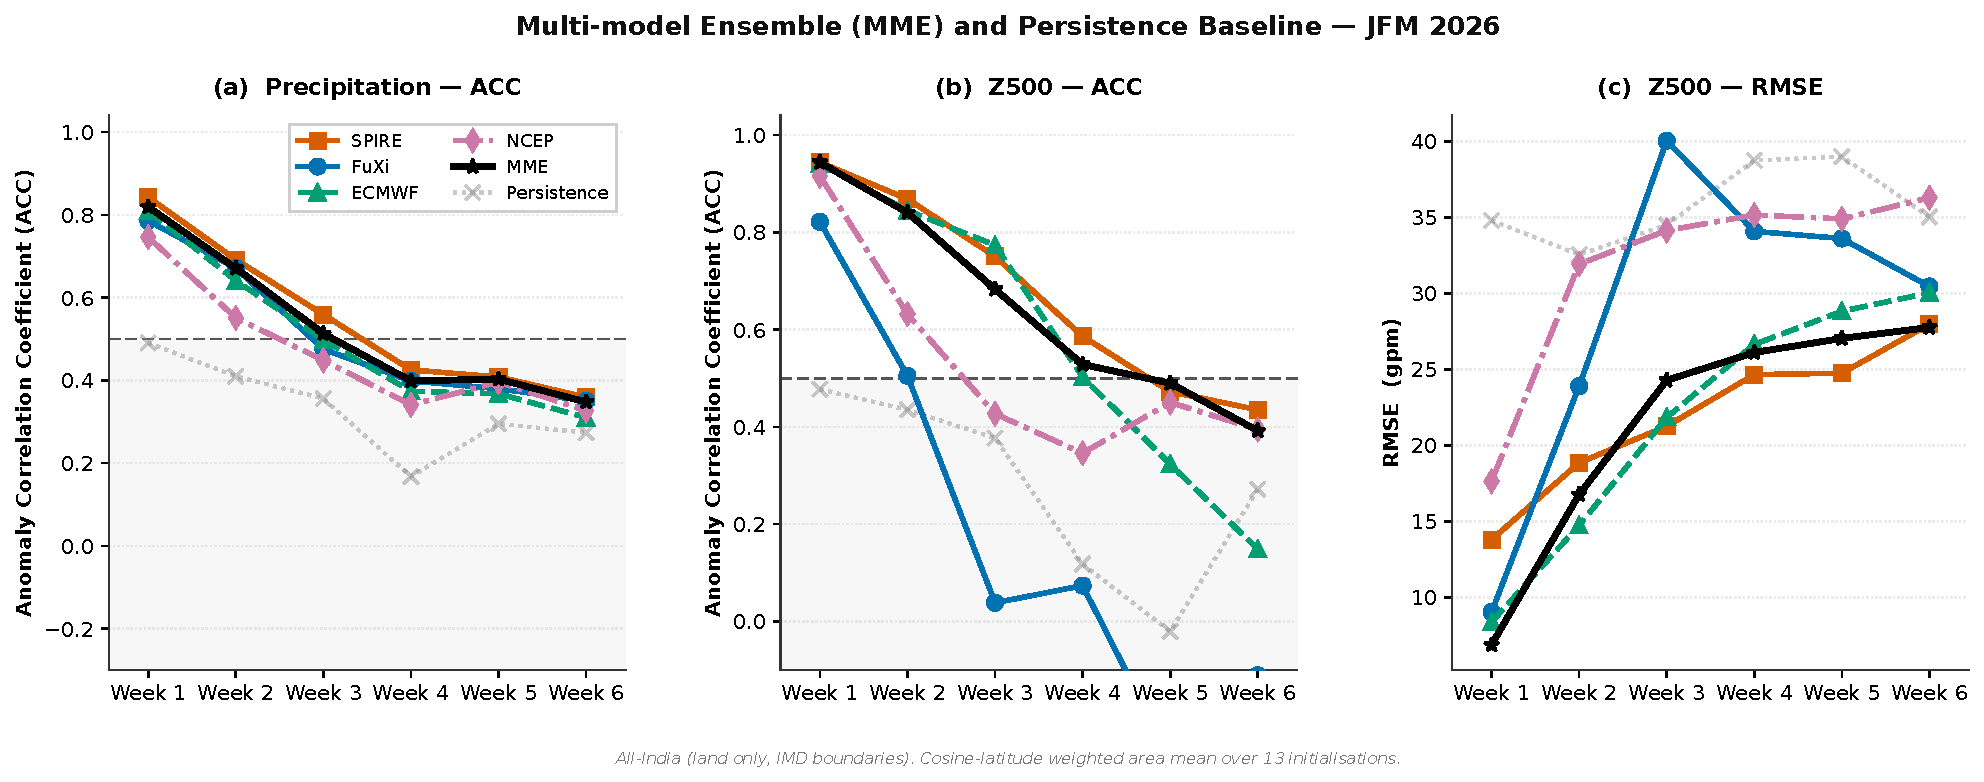
\includegraphics[width=\linewidth]{figs/fig06_mme_persistence.pdf}
  \caption{All-India area-averaged weekly anomaly versus lead week for
  (a)~precipitation and (b)~Z500, averaged over the 13 JFM~2026
  initializations. Each coloured line is an individual system's ensemble
  mean; the dashed lines are the multi-model ensemble (MME) mean and the
  persistence baseline. ERA5 weekly anomaly is in black. Shading shows
  the $\pm1\sigma$ spread range for SPIRE.}
  \label{fig:mme}
\end{figure*}

\begin{figure*}[htbp]
  \centering
  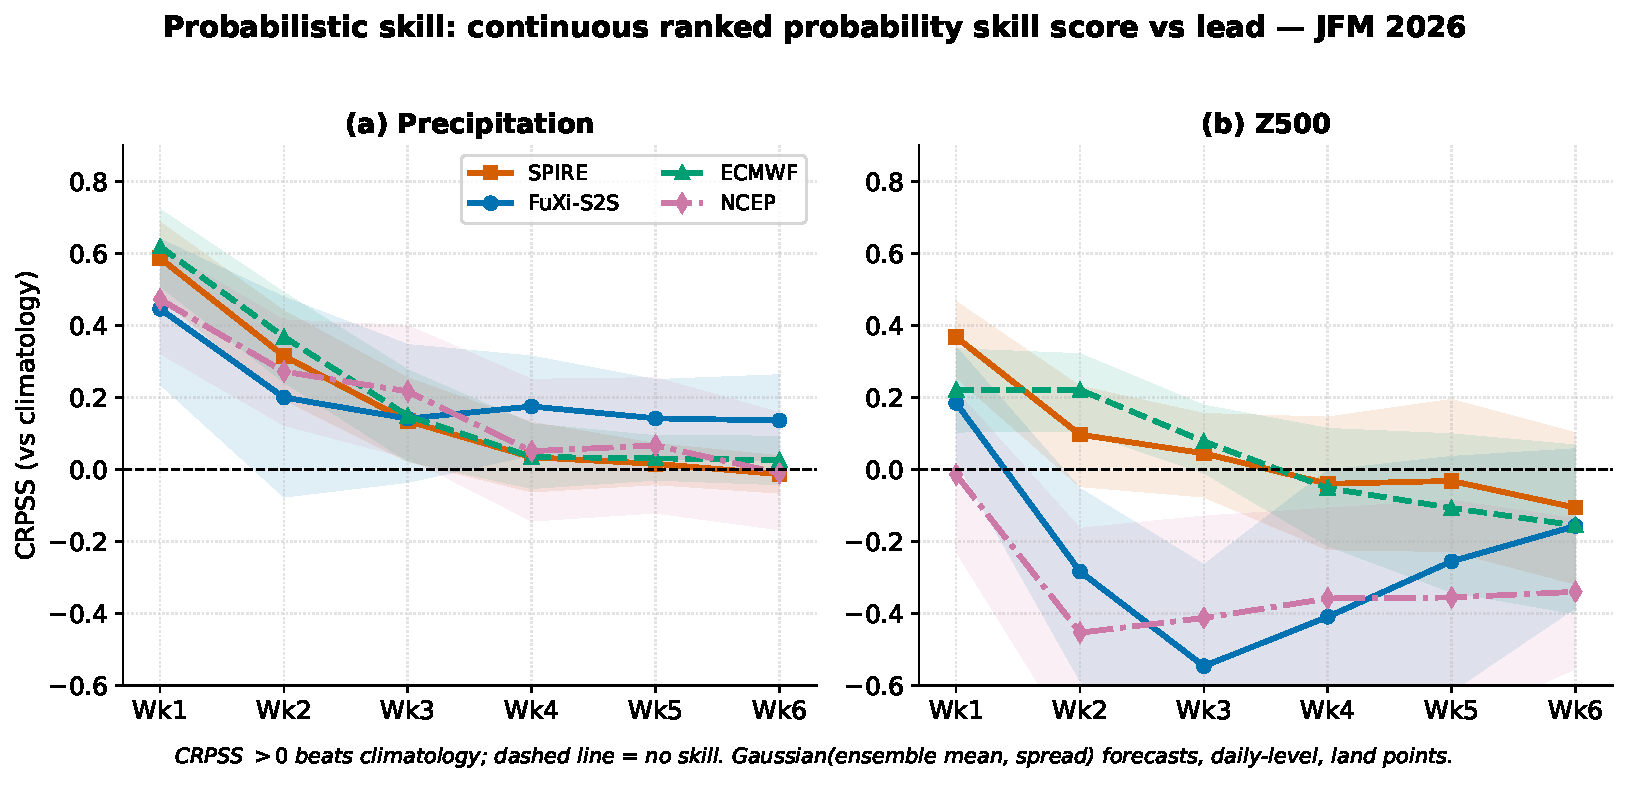
\includegraphics[width=\linewidth]{figs/fig15_crpss.pdf}
  \caption{Continuous Ranked Probability Skill Score (CRPSS) versus lead
  week for (a)~precipitation and (b)~Z500, averaged over the 13 JFM~2026
  initializations and all India land points. Positive values indicate skill
  above climatology; the dashed line marks CRPSS${=}0$. Bootstrap 95\%
  confidence intervals across initializations are shown as shading.}
  \label{fig:crpss}
\end{figure*}

\begin{figure*}[htbp]
  \centering
  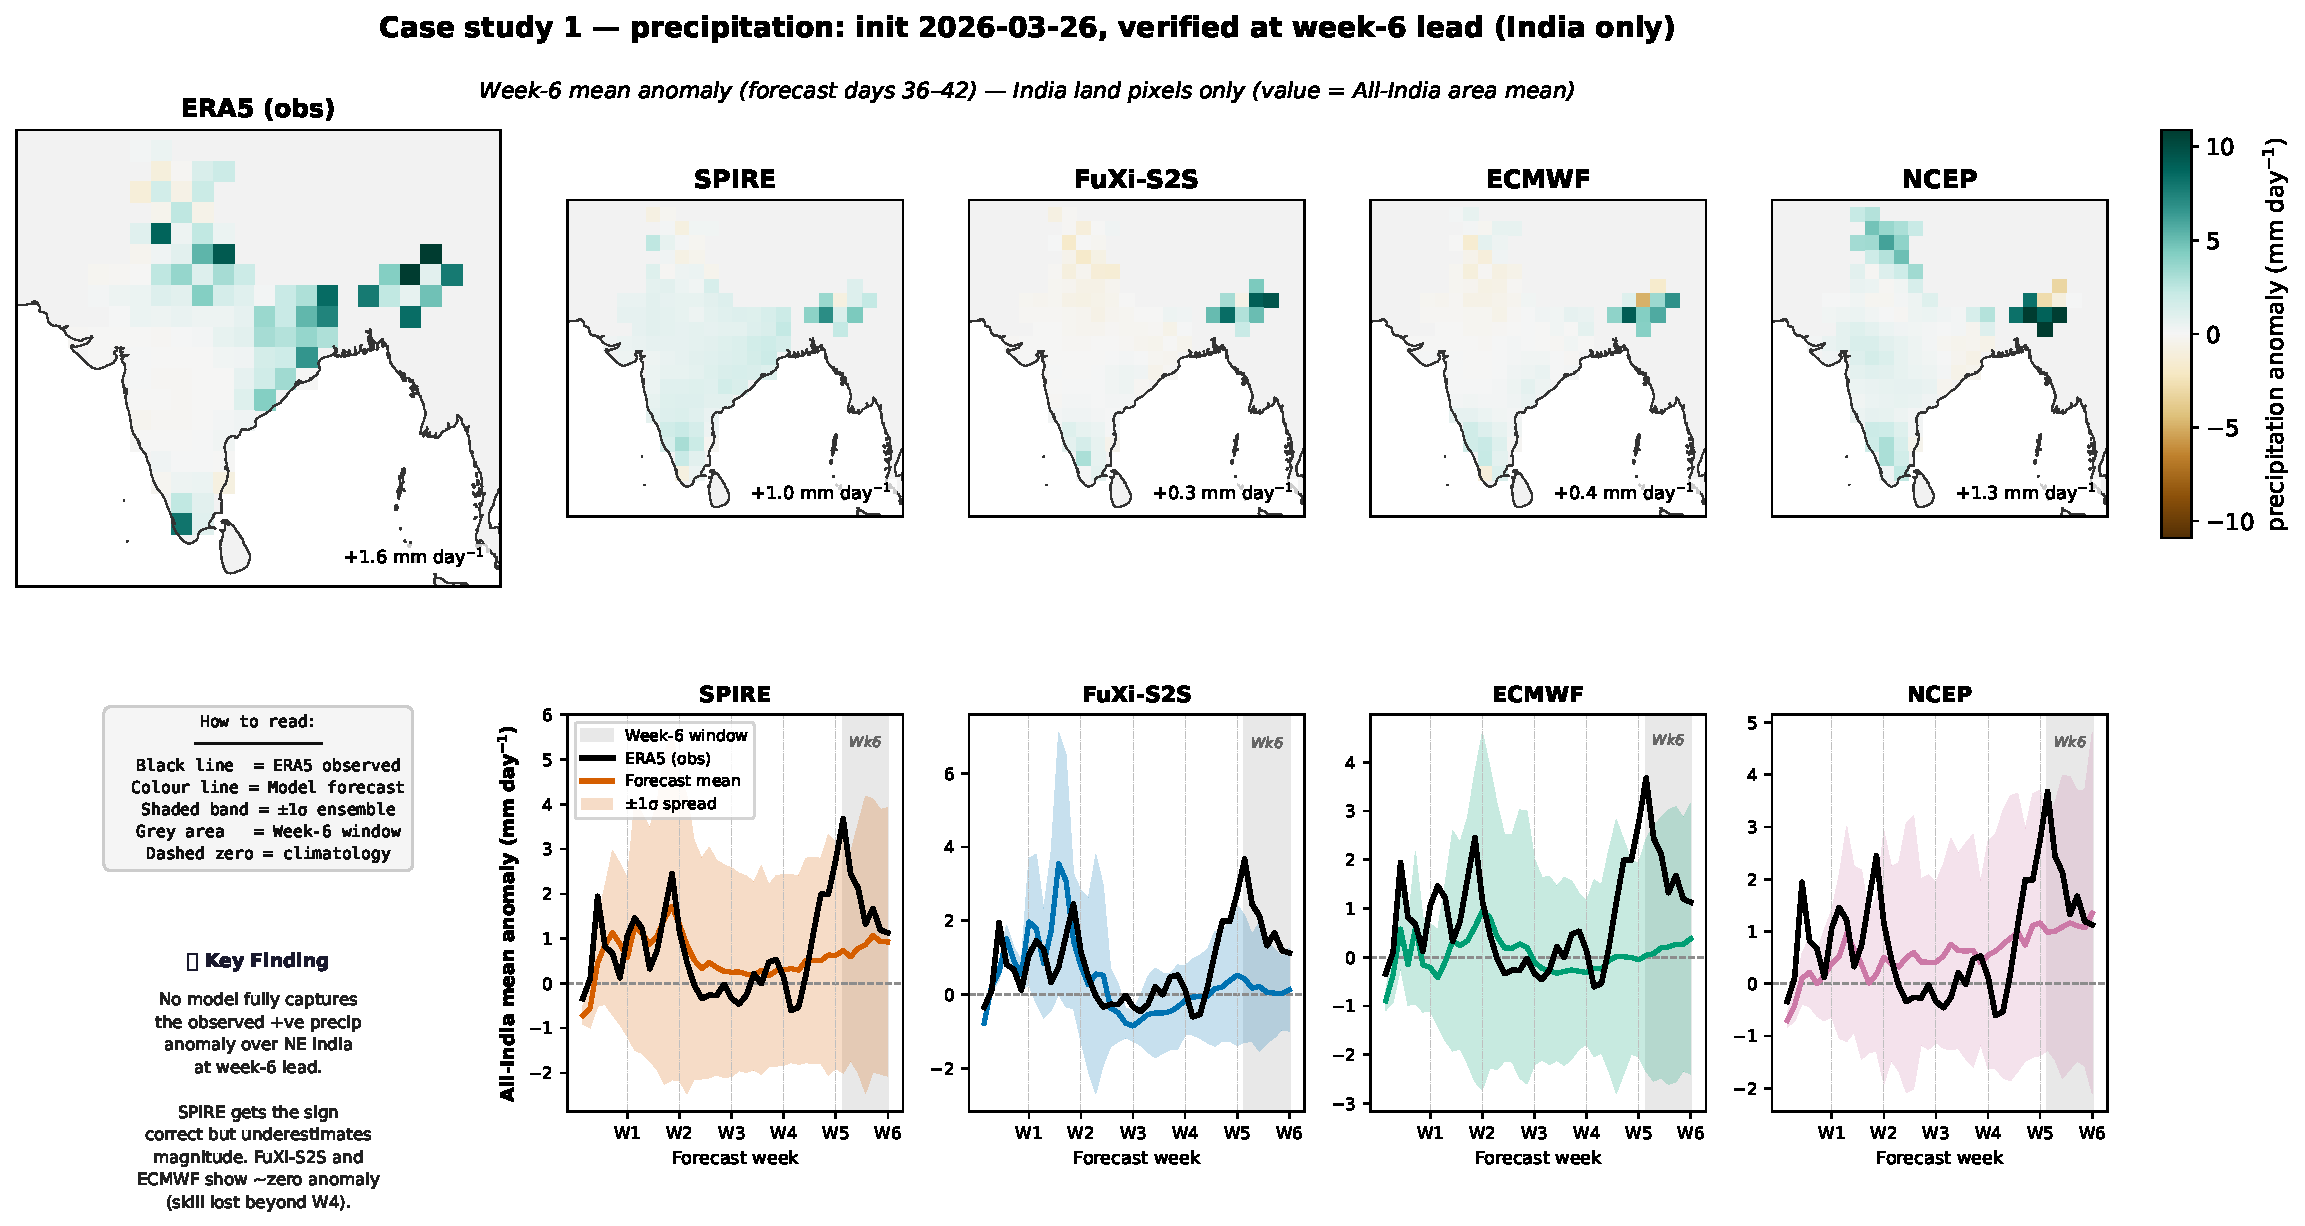
\includegraphics[width=\linewidth]{figs/fig20_casestudy_precip.pdf}
  \caption{Week-6 case study: \textbf{precipitation} (mm\,day$^{-1}$),
  initialization 26~March~2026. Top row: ERA5 observed weekly mean
  anomaly. Subsequent rows: ensemble-mean forecast anomaly for each
  system. The dry anomaly over northwestern India and wet anomaly over
  the peninsula are the principal features of interest.
  Ocean points masked; coastline shown.}
  \label{fig:case_precip}
\end{figure*}

\begin{figure*}[htbp]
  \centering
  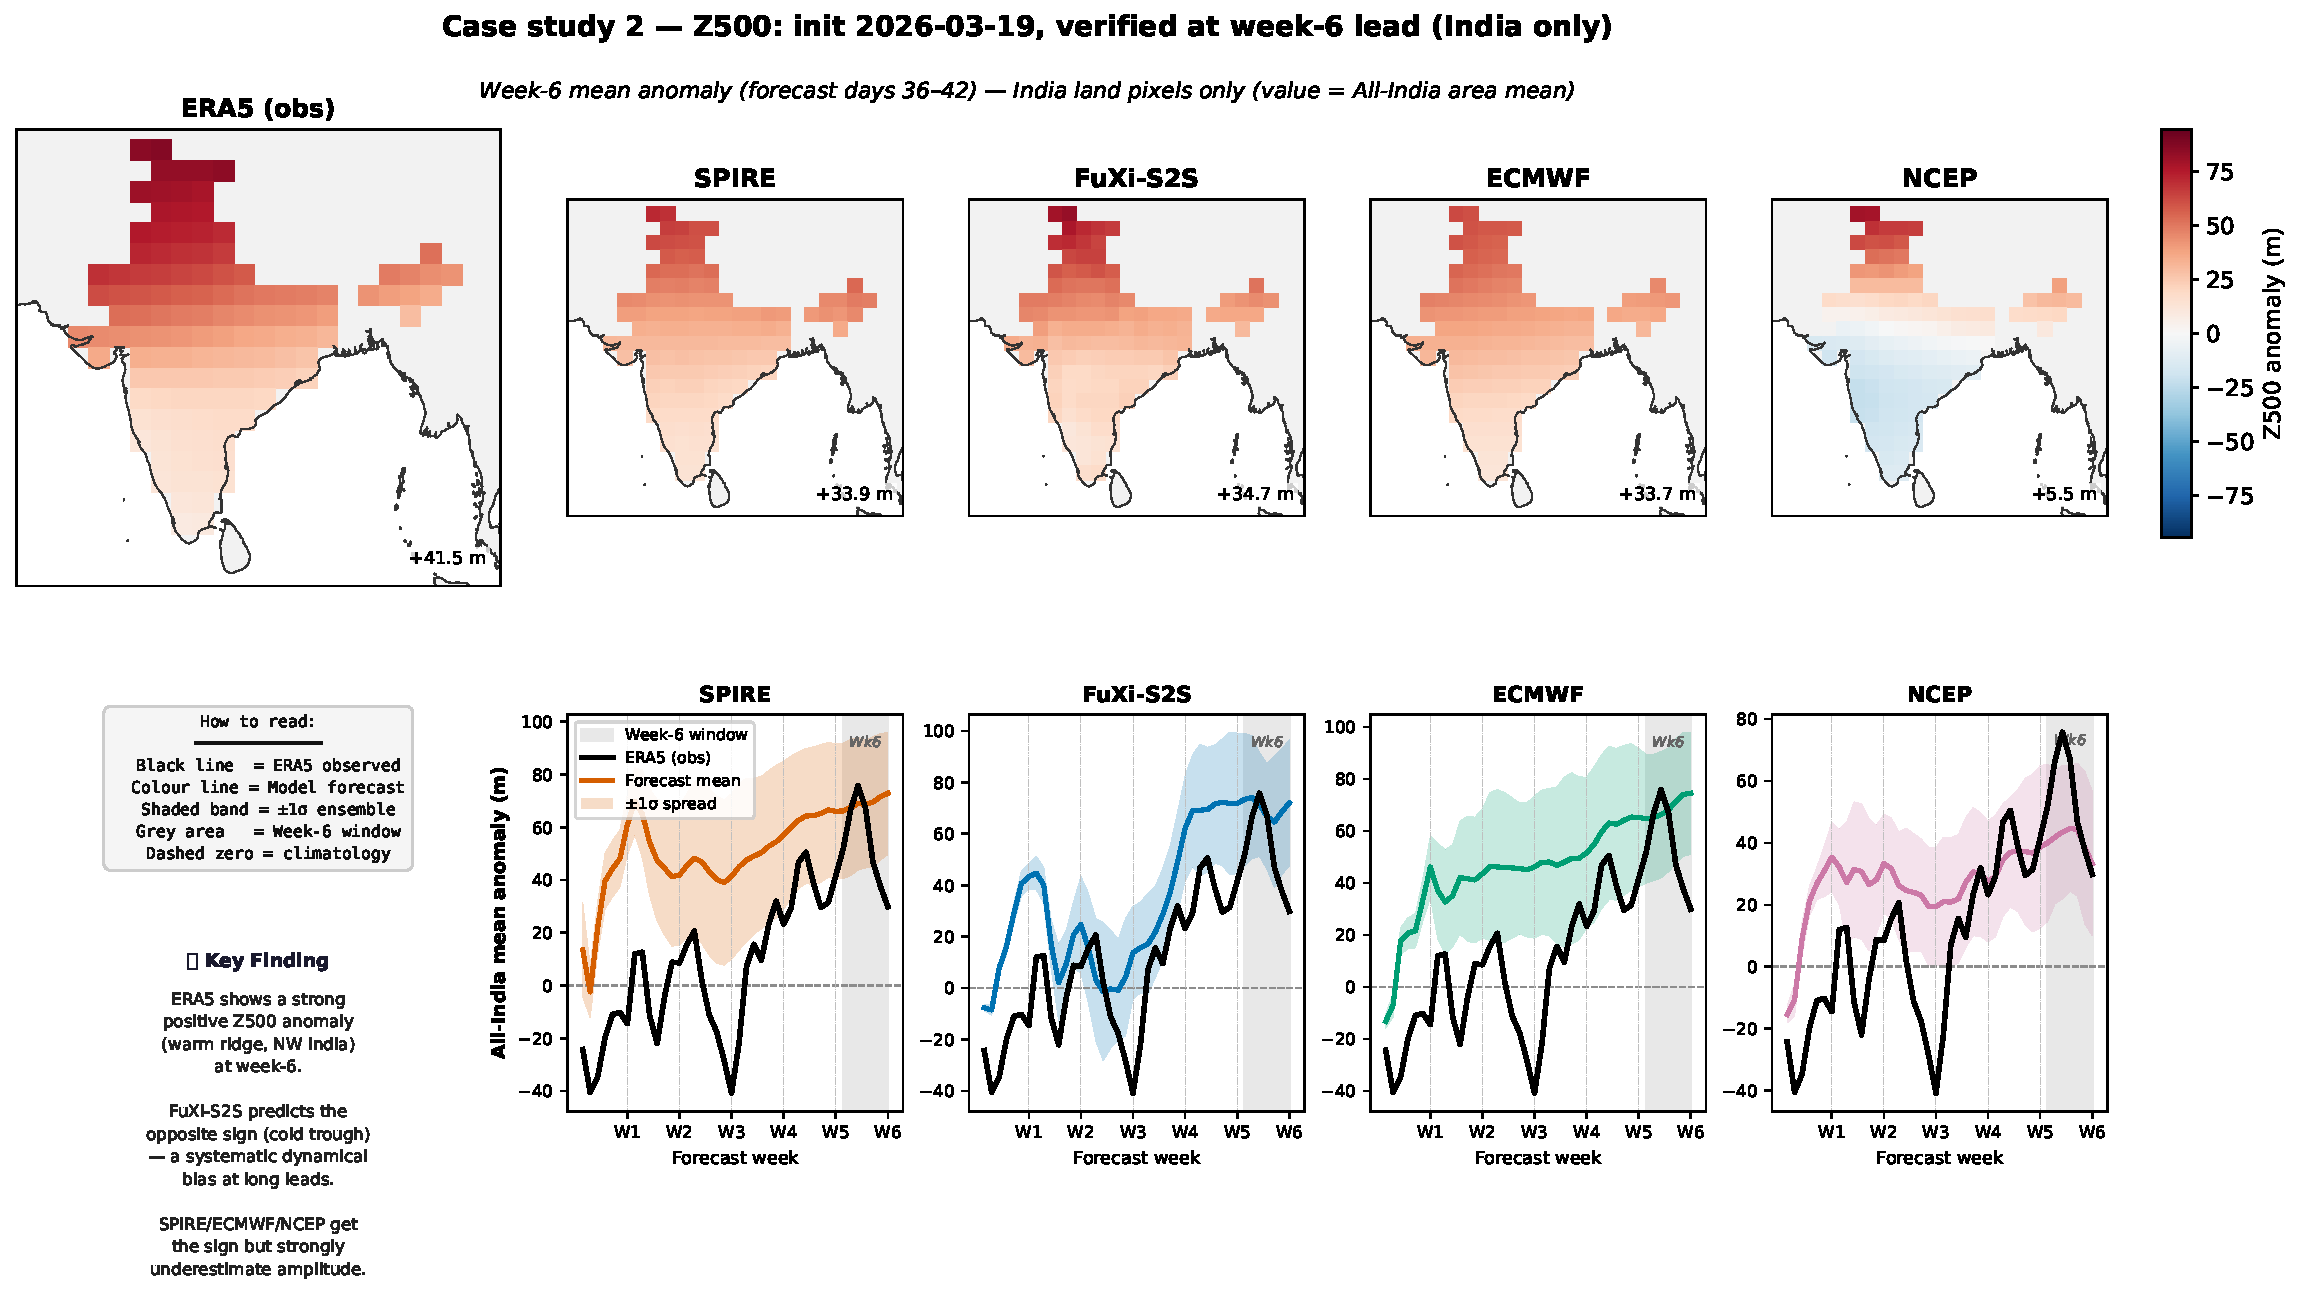
\includegraphics[width=\linewidth]{figs/fig21_casestudy_z500.pdf}
  \caption{As Fig.~\ref{fig:case_precip} but for the week-6
  \textbf{Z500 anomaly} (m), initialization 26~March~2026.
  The observed ridge over central Asia and trough over the Bay of
  Bengal are largely missed by NCEP and FuXi-S2S at this lead.
  Ocean points masked; coastline shown.}
  \label{fig:case_z500}
\end{figure*}

\begin{figure*}[htbp]
  \centering
  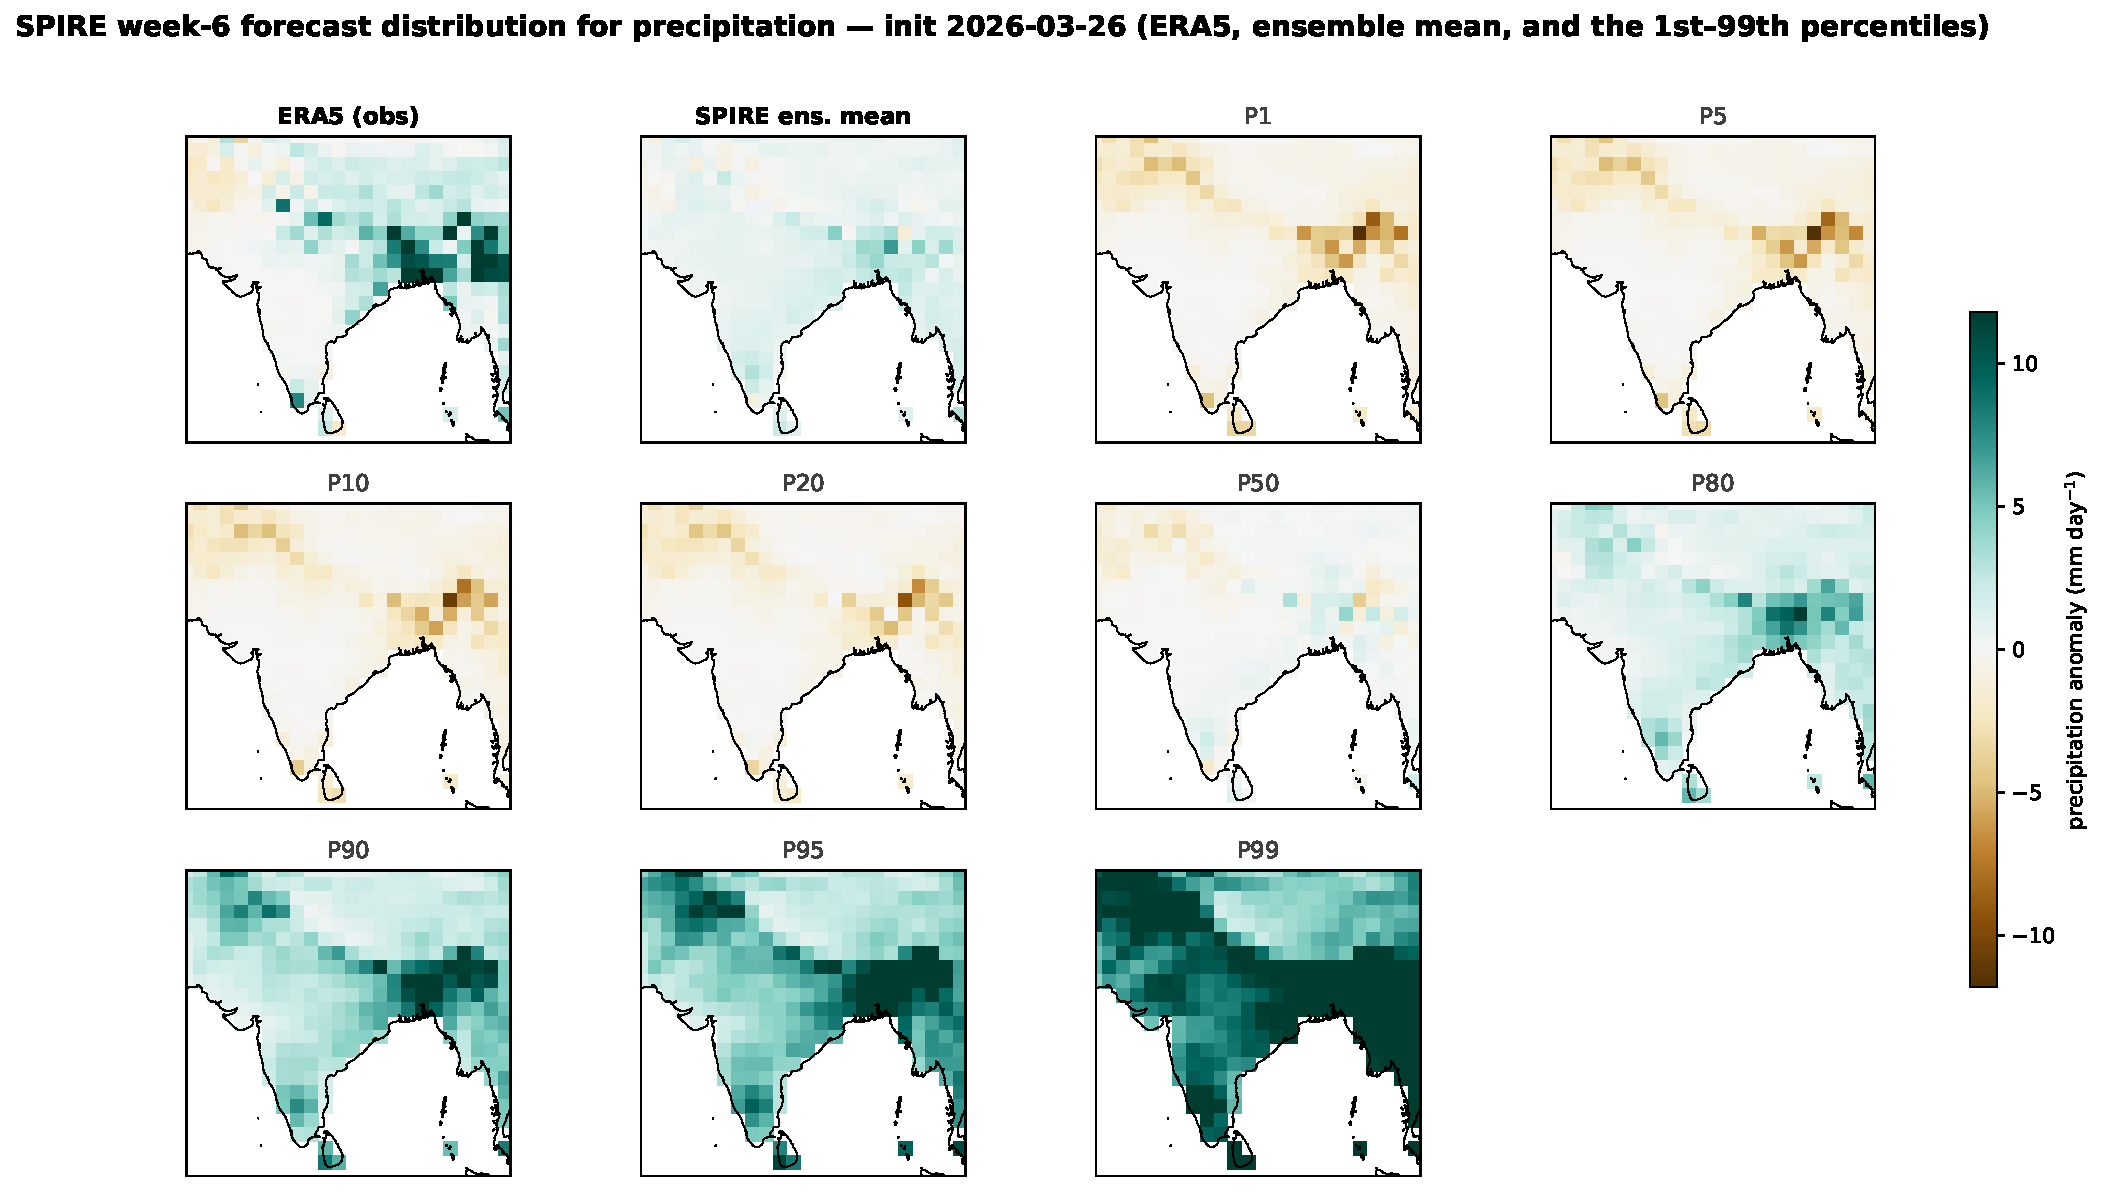
\includegraphics[width=\linewidth]{figs/fig27_spire_gallery_precip.pdf}
  \caption{SPIRE forecast percentile distribution for the week-6
  \textbf{precipitation} case study (initialization 26~March~2026).
  Panels show the ERA5 observed anomaly, the SPIRE ensemble-mean
  anomaly, and selected percentile anomaly maps (P1, P5, P10, P20,
  P50, P80, P90, P95, P99) across the six forecast weeks. SPIRE
  delivers distribution percentiles rather than individual members.
  Ocean masked; coastline shown.}
  \label{fig:gallery_t2m}% alias kept for cross-ref compatibility
  \label{fig:gallery_precip}
\end{figure*}

\begin{figure*}[htbp]
  \centering
  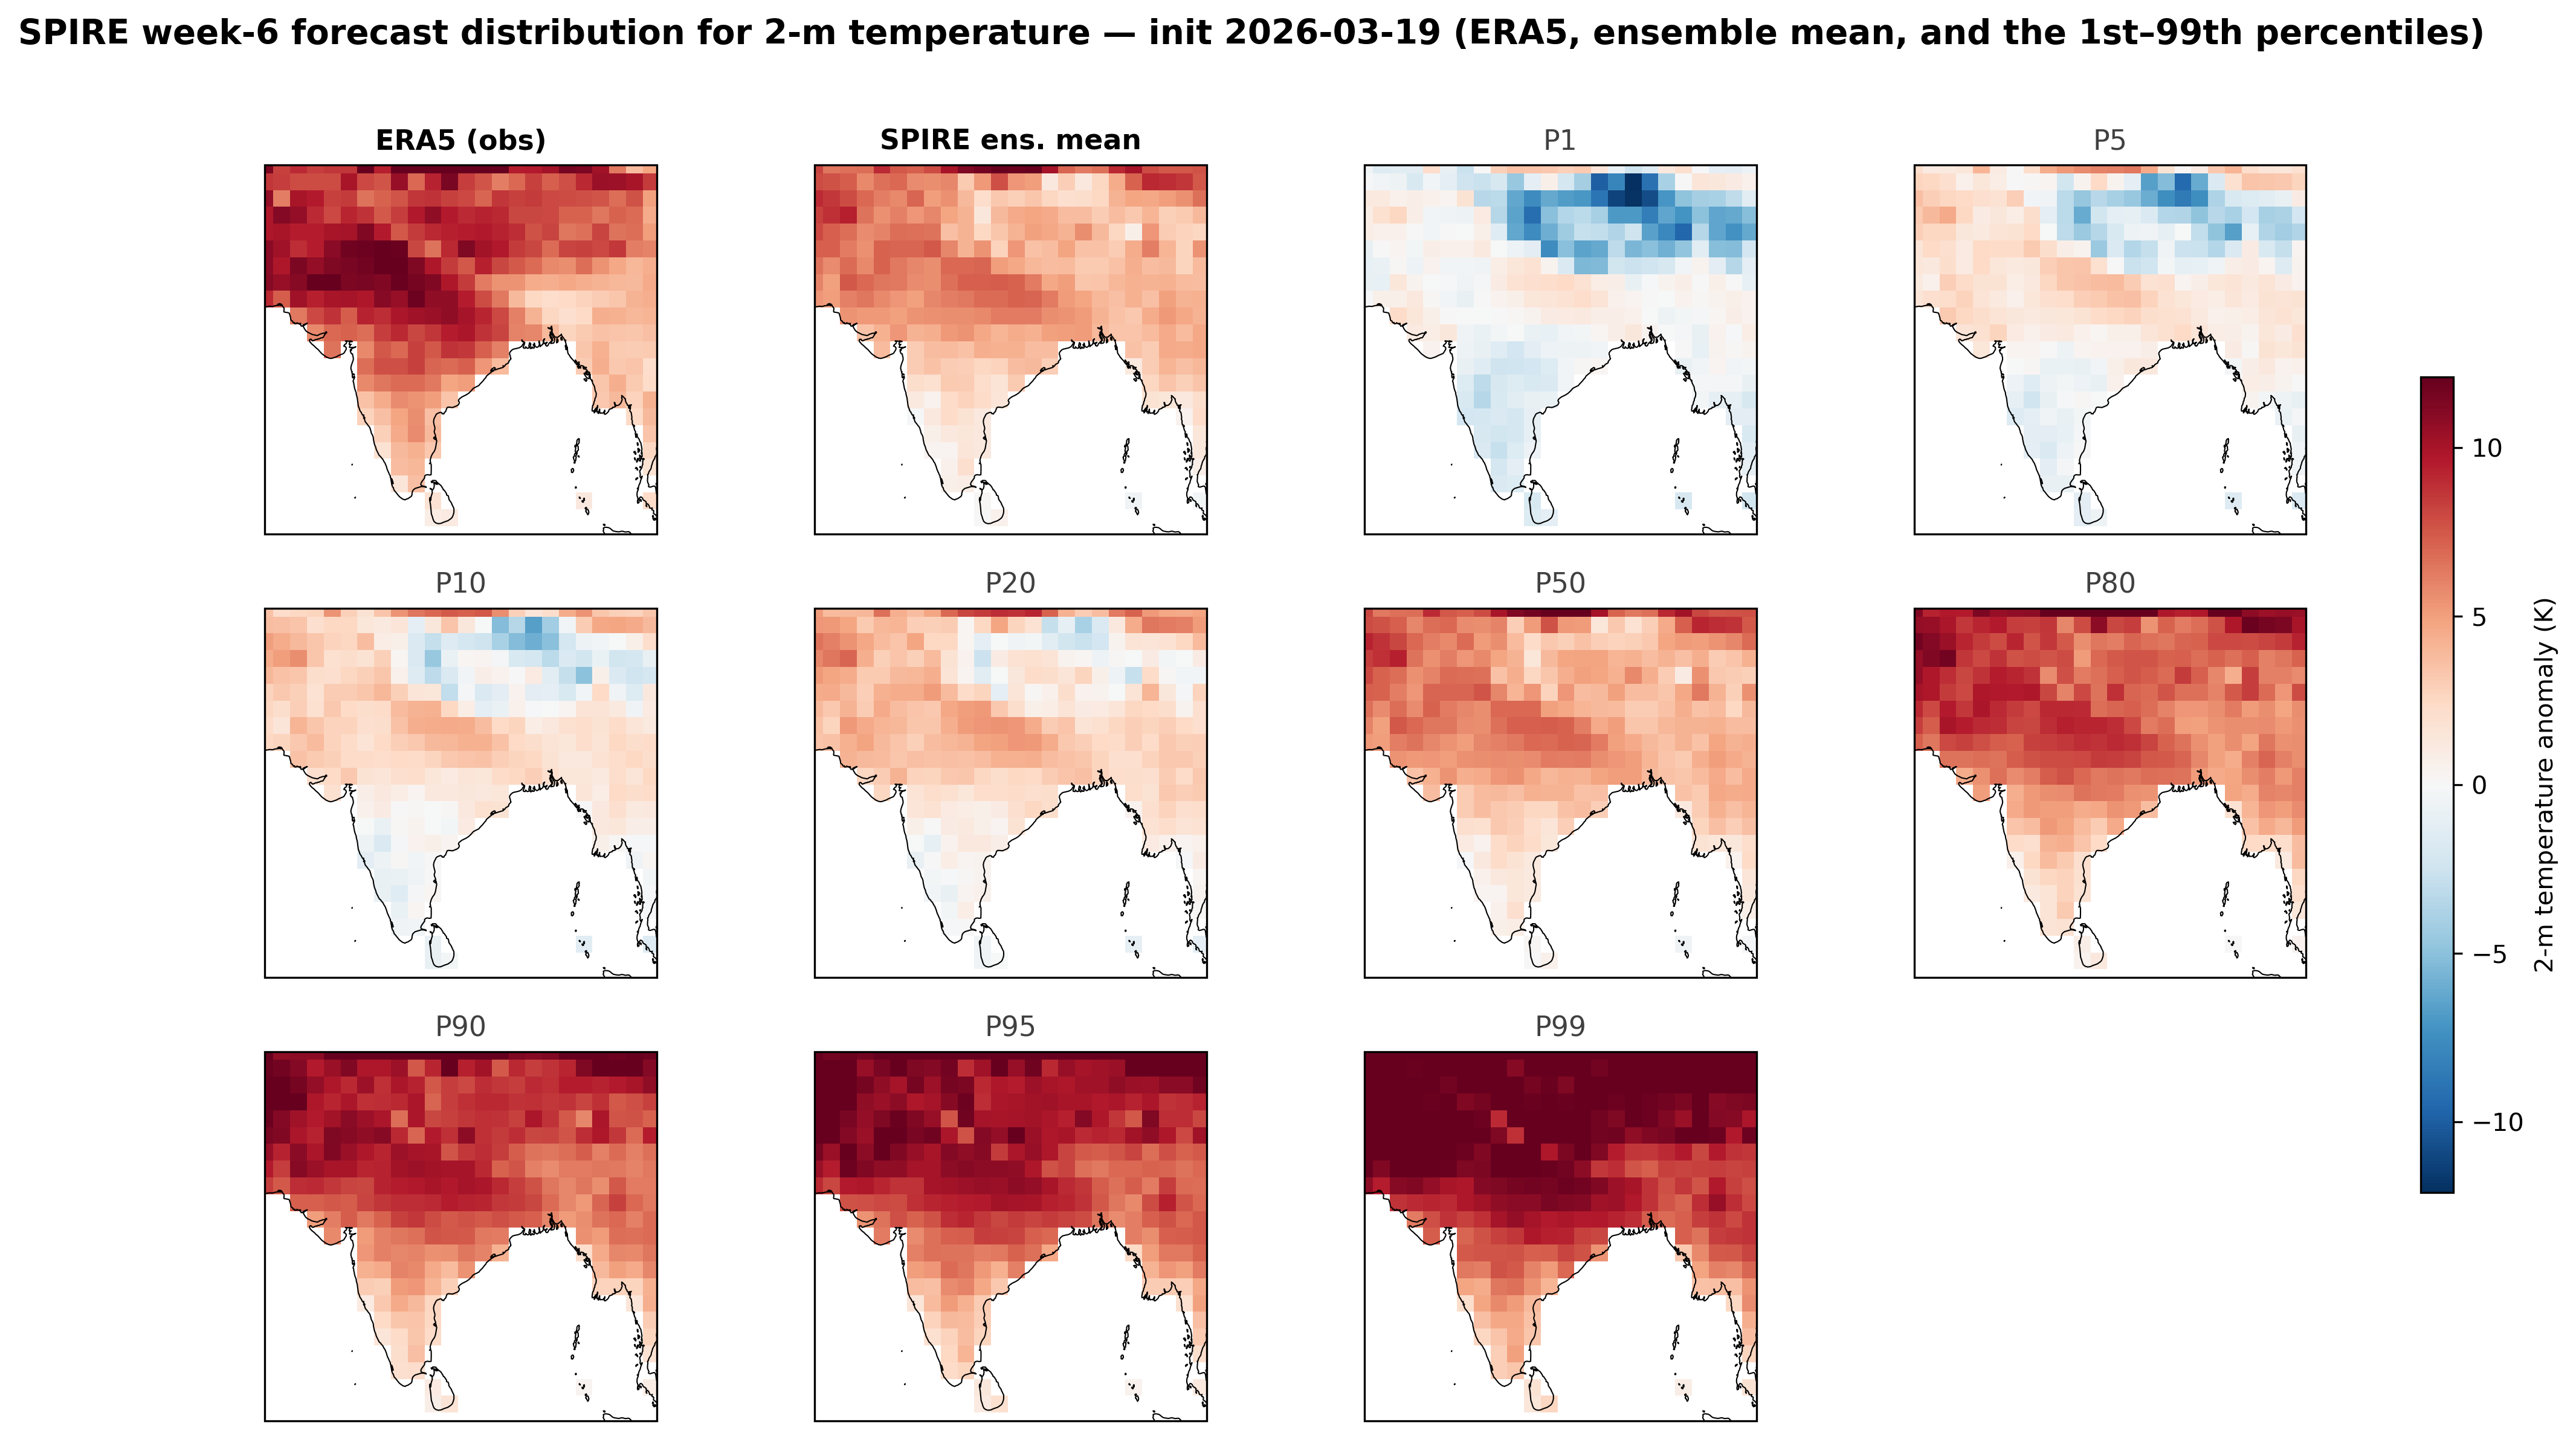
\includegraphics[width=\linewidth]{figs/fig26_spire_gallery_t2m.png}
  \caption{SPIRE forecast percentile distribution for the week-6
  \textbf{2-m temperature} case study (initialization 19~March~2026).
  Panels show the ERA5 observed 2-m temperature anomaly (K), the SPIRE
  ensemble-mean anomaly, and selected percentiles (P1--P99).
  The broad warm anomaly over northern and central India is captured in
  the upper percentiles, while the lower tail spans near-neutral
  conditions, illustrating the full probabilistic range at week-6 lead.
  Ocean masked; coastline shown.}
  \label{fig:gallery_t2m2m}
\end{figure*}

\end{document}
